\chapter{Analysis}

\section{Normalization of Relative Yields}

The base measurement for the studies presented in this paper is, fundamentally, the number of dimuon events on a given target. This is known as the \emph{raw yield} (Y). The ratio of these yields for a given target is used to study the kinematic dependence of the \emph{per nucleon cross section ratio} that defines these phenomenon, but there must be a target-to-target normalization for such measurements.
\begin{equation}
R \equiv \frac{F_2^A}{F_2^D} \approx \frac{\sigma_{\mu\mu}^A}{\sigma_{\mu\mu}^D} \frac{2}{A} = N_{A/D} \frac{Y^A}{Y^D}
\end{equation}
Here, $A$ is the mass number of the target nucleus, and $N_{A/D}$ is the normalization factor, which can be expressed as:
\begin{equation}
	N_{A/D} =
		\left(\frac{ N_0^D \cdot \text{lt}^D \cdot T^D(\xi)}{N_0^A \cdot \text{lt}^A \cdot T^A(\xi) } \right) \cdot 
		\left( \frac{ 2 \cdot n_D \cdot L^D }{ A \cdot n_A \cdot L^A } \right) \cdot 
		\frac{ \varepsilon^D }{ \varepsilon^A }  \cdot 
		\frac{ \bar{\Omega}^D }{\bar{ \Omega}^A } \cdot 
		\frac{ \epsilon^D }{ \epsilon^A }
\end{equation}
where $N_0$ is the number of incident protons, \emph{lt}$^A$ is the \% live time on the target, $T^A$ is the target transmission (or beam attenuation) factor, $n_A$ is the number of nuclei per unit volume, $L^A$ is the target thickness, $\varepsilon^A$ is the detector efficiency, $\bar{\Omega}^A$ is the spectrometer acceptance, and $\epsilon^A$ is the tracking reconstruction efficiency. One of the key benefits of performing a ratio measurement is that, to good approximation, the terms regarding chamber efficiency, tracking efficiency, and acceptance should be equal across targets and should therefore cancel each other out. How well this assumption holds up will be assessed and evaluated.

With the normalization applied, this ratio $R$ can be accurately studied by being binned in one or more kinematics in order to observe interesting behaviors and compare them against previous measurements and various models. Once The cuts described in the previous section are applied, the surviving dimuons are all considered to be \emph{good quality target Drell-Yan dimuons}, and all analyses and corrections described from here on refer to them only.

This section will discuss the several components of the target-to-target relative normalization from the determination of beam intensity, target thickness, live time, chamber efficiency, and acceptance. Beam intensity and live time information was obtained from the BIM and scaler data. Acceptance was calculated with Monte Carlo simulation. Finally, chamber efficiencies and their ratios per target were studied with NIM3 random trigger data embedded onto clean MC. The tracking efficiencies are highly rate-dependent, and will be discussed at length in another section.

\subsection{Live Proton Count and Beam Attenuation}

The measurements of the number of incident protons, live time, and beam attenuation combine to give a figure for the total number of protons on target for which data was recorded. The important sources to consider here are the upstream SEM detectors that record the number of incident protons, the QIE recorded sums of protons (in QIE units), the number of QIE units for which there was either a trigger inhibit or DAQ deadtime. In practice, SeaQuest calculates a value called ``live protons'' \emph{for each spill}:
\begin{equation}
 N_0^A = \text{G2SEM}\ \ \ ;\ \ \ \text{lt}_A = 
 \frac{\text{QIESum} - \text{inhibit} - \text{deadtime}}{\text{QIESum}}\ \ \ ;\ \ \ 
 liveProton = N_0^A \cdot \text{lt}_A
\end{equation}
this \emph{liveProton} value is integrated, good spill by good spill, for every target in each data set.

\red{What are average livetimes for the experiment? Deviations?}

It is also important to factor in the effects of inelastic scattering of the beam within the target, causing the effective amount of beam-on-target to decrease with every step $dz$ through the target. This is different for each target based on target nuclear densities and cross sections. With this, the liveProton value can be corrected. Consider incident proton number $N_0$, where $dN$ is the number of protons attenuated when passing through target slice $dz$, and $L$ is the total length of the target. The function for the number of protons remaining at a given position $z$ is
\begin{equation}
 N(z) = N_0 e^{-\frac{\rho_A}{\text{NIL}_A} z} = N_0 e^{-z/\lambda}
\end{equation}
where $\rho_A$ is the density of the material, $\text{NIL}_A$ is the nuclear interaction length of the target, and $\lambda = \frac{\text{NIL}_A}{\rho_A}$. When integrating over the length of the target, one arrives at the total [$\text{protons}\cdot \text{cm}$] exposed to the target. Assuming that each proton interacts independently, one can divide this integral by the length of the target to arrive at \emph{effective} number of protons incident on the target
\begin{equation}
N_{\text{eff}} = \frac{1}{L} \left[ N_0 \lambda (1 - e^{-\frac{L}{\lambda}})\right] = N_0 \left[\frac{1 - e^{-\xi}}{\xi}\right] =  N_0 T(\xi)\ \ \ ;\ \ \ 
\xi = L/\lambda.
\end{equation}
The normalization of the transmission or beam attenuation factor $T^D/T^A$ is therefore only a function of the length of the target, its density, and its nuclear interaction length. In total, the product of $N_0 \cdot \text{lt} \cdot T(\xi)$ represents the effective protons on target which was recorded by the data acquisition systems. Values of $\xi$ and $T(\xi)$ can be found in Table~\ref{tab:targ-details}.

\subsection{Target Density Ratios}

The number of nucleons that the effective protons will interactive should be considered when performing the target-to-target normalization. Aside from the background ``targets'' and liquid hydrogen, there are four nuclear targets in this A-dependence study. The nucleons in liquid deuterium are viewed as essentially free particles, and therefore proved an isoscalar reference by which the heavier targets are compared to. In all, the nuclear targets used are $D_2$, C, Fe, and W, and their attributes pertinent to target density ratios can be found in Table~\ref{tab:targ-details}. The yield ratios are normalized to the number of nucleons in each target by the normalization component $(2 \cdot n_D \cdot L^D) / (A \cdot n_A \cdot L^A)$. 

\begin{table}
	\centering
\begin{tabular}{lrrrrrrrr}
	\toprule
	{} &  Target &  Length[cm] & $n_A$ [mol/cm$^3$] & $\rho$ [g/cm$^3$] &  NIL [g/cm$^2$] &   $\lambda$ [cm] & $\xi$ & T($\xi$) \\
	Target & Position & & & & & & & \\
	\midrule
	$D_2$ & 3 & 50.80 & 0.081 & 0.163 & 71.8 & 439.41 & 0.1156 & 0.944 \\
	Fe & 5 & 1.91 &	0.141 & 7.874 & 132.1 & 16.78 & 0.1136 & 0.945 \\
	C & 6 & 3.32 & 0.150 & 1.802 & 85.8 & 47.61 & 0.0698 & 0.966 \\
	W & 7 & 0.95 & 0.105 & 19.300 & 191.9 & 9.94 & 0.0958 & 0.954 \\
	\bottomrule
\end{tabular}
\caption{Details pertaining to the measurables and physical properties individual nuclear targets.}
\label{tab:targ-details}
\end{table}

\red{Uncertainties in densities, target lengths? Find solid target with largest uncertainty, estimate LD2 uncertainty the best we can, get \% systematic from the ratio of them.}

\subsection{Detector Efficiency}

The key cause of detector inefficiency is high occupancies from high intensity events. Also, the total number of tracks that fired off elements of the many detectors is dominated by events generated from the \unit[503]{cm} iron beam dump. The difference in interaction lengths of the targets should have only a small effect on the absolute chamber and hodoscope efficiencies~\red{show plot of efficiencies}. Further, any longer term time-dependent drifts in detector efficiencies will largely cancel out due to the frequent minute-by-minute interchange of targets. It is therefore justifiable to assume that there is no target-to-target chamber efficiency dependence to normalize to. The overall ratio of detector efficiencies between targets is therefore taken to be $\varepsilon^D/\varepsilon^A=1$. 

It is however possible that pions created in the targets have more of a chance to decay into muons that proceed to add to the background hit rates of the experiment; pions created in the beam dump are much more likely to get re-absorbed before they decay. To investigate the possible magnitude of this contribution to occupancy, detector occupancies were studied for the different targets in unbiased NIM3 random events as a function of chamber intensity. We see in Figure~\ref{fig:occ-int-targ} that they are not significantly different from each other, though there is a slight difference in occupancies between the deuterium target and the rest. However, since the occupancy distributions at a given intensity bin do not change much for a given intensity, it is safe to assume that the efficiencies likewise do not change by much from target-to-target.
\begin{figure}
	\centering
	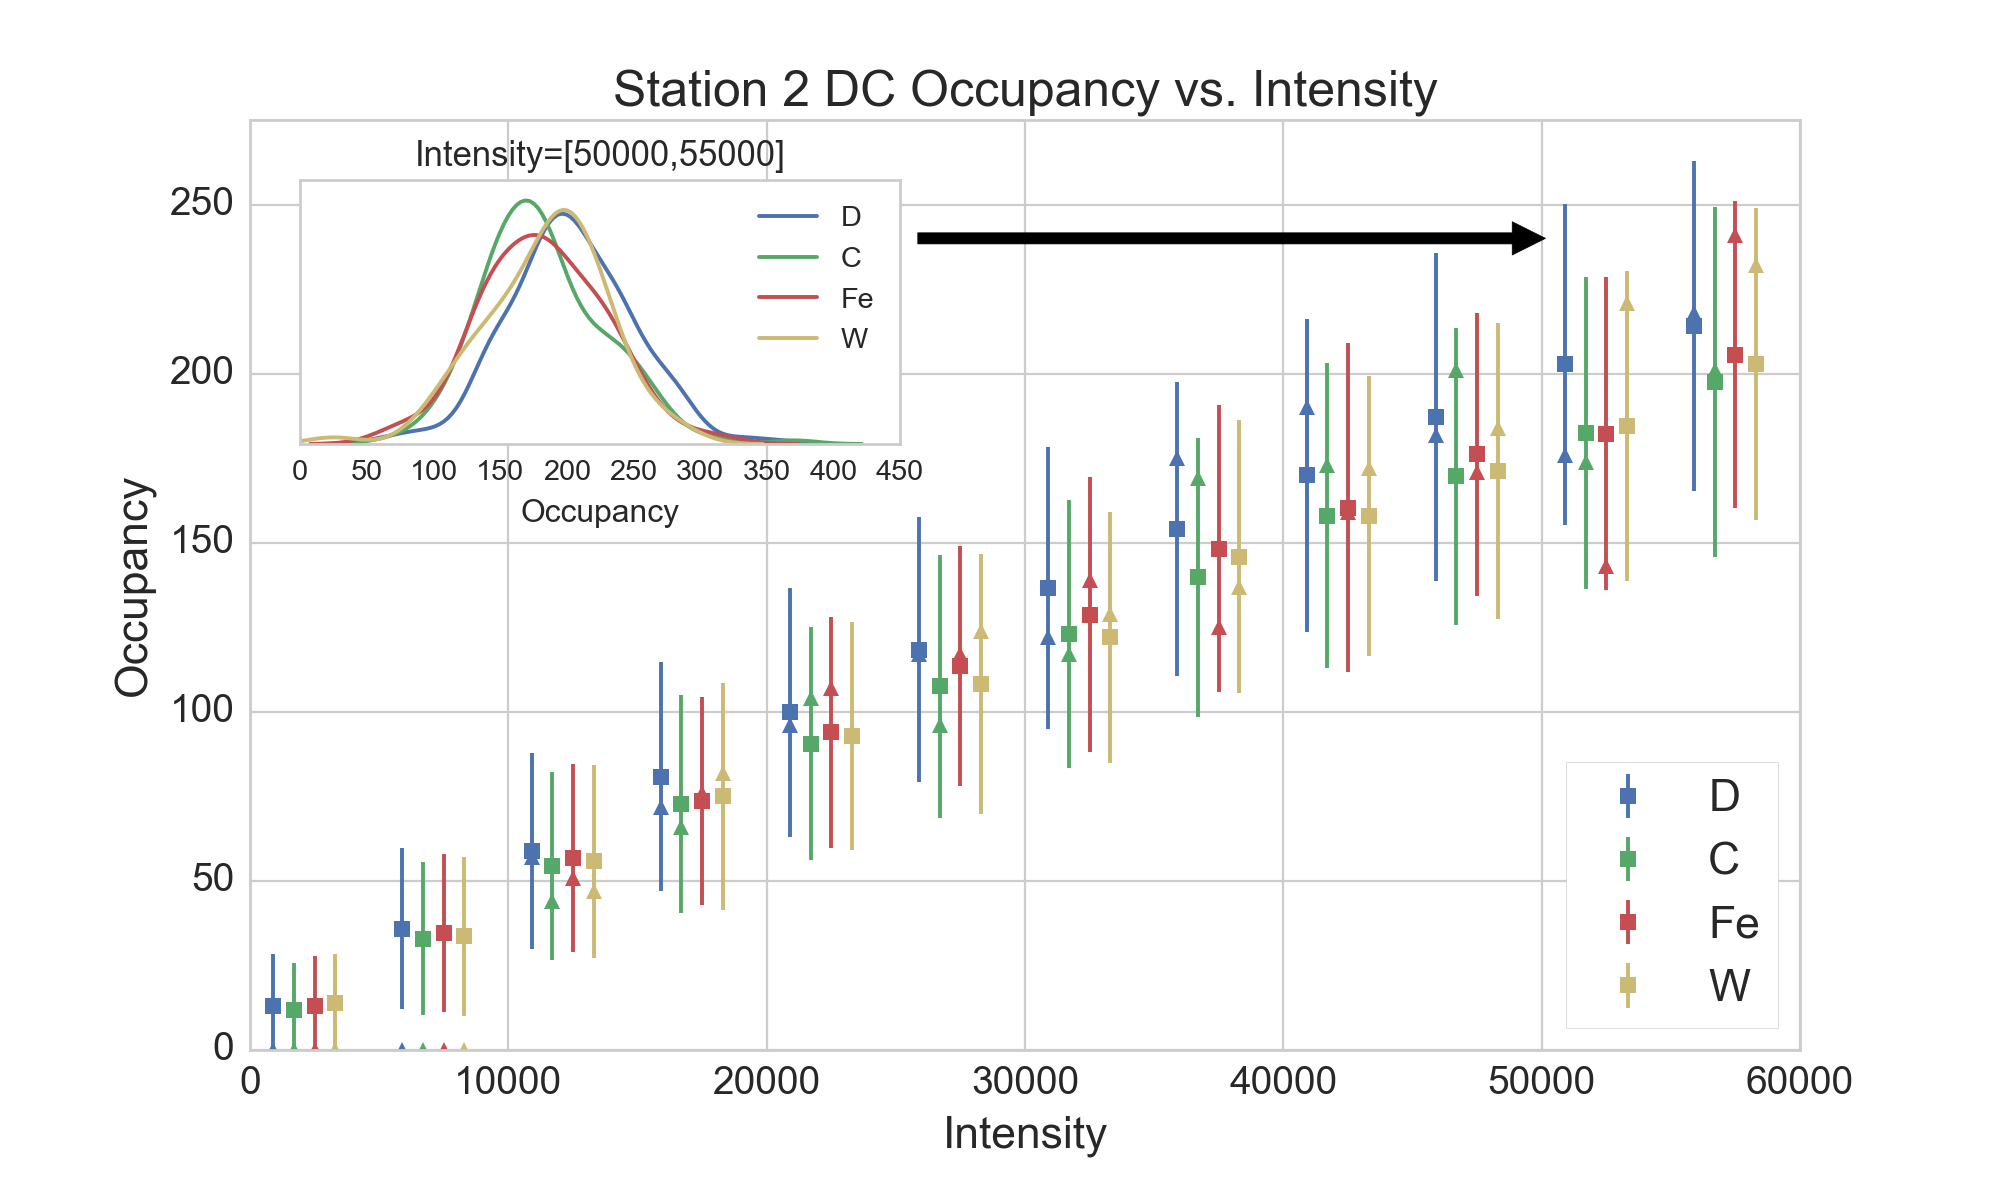
\includegraphics[width=5in]{figures/analysis/targ-occupancy.png}
	\caption{The Station 2 drift chamber occupancy for the four targets as a function of intensity. The error bars show a systematic deviation of occupancies from the mean for a given intensity bin. The inset plot shows a KDE plot of distributions for the intensity bin in which the values differ the most. The triangle markers represent the modes of the distributions.}
	\label{fig:occ-int-targ}
\end{figure}

To override any concern of chamber efficiencies having an effect on any absolute or ratio measurements, a study was performed to measure the effect of chamber efficiencies on the track reconstruction algorithm. This was done by embedding clean Monte Carlo-generated Drell-Yan dimuons into real NIM3 random event hit data. Then, a constant 94\% chamber efficiency was applied by removing a random 6\% of the chamber hits, and tracking was performed on this sample. The 94\% figure reflects the best estimate of overall chamber efficiencies at SeaQuest. Following that, a rate-dependent chamber efficiency was imposed of the form
\begin{equation}
\varepsilon(I) = 0.95 - a \cdot I
\end{equation}
where $a$ was set to \unit[2e-6]{protons$^{-1}$}. This resulted in a linear drop in efficiency with it dropping to as low as 75\% at the highest intensity regions considered (\unit[100000]{protons}). The tracking algorithm was then run on this data sample.
	
For even the constant 94\% efficiency case, the tracking is expected to decrease in \emph{tracking efficiency} (a very different topic to tackle, as we will approach later in this chapter) as intensity increases and pattern recognition becomes more difficult as overall occupancies increase. The important to observation to make is how this intensity-dependent tracking efficiency compares to the case of decreasing efficiency. For both cases, the ratio of successful reconstructions to all thrown dimuons (before even the trigger acceptance is imposed) can be seen in Figure~\ref{fig:ktrack-eff-int}. It is perhaps surprising to see that even at high intensities, the linear drop in tracking efficiencies does not change between the two cases. The reason for this is due to the fact that the tracking algorithm is very \emph{robust} in the way it is able to handle missing hits, as it only requires a few hits in each station (3 out of 6) to successfully find a track.
\begin{figure}
	\centering
	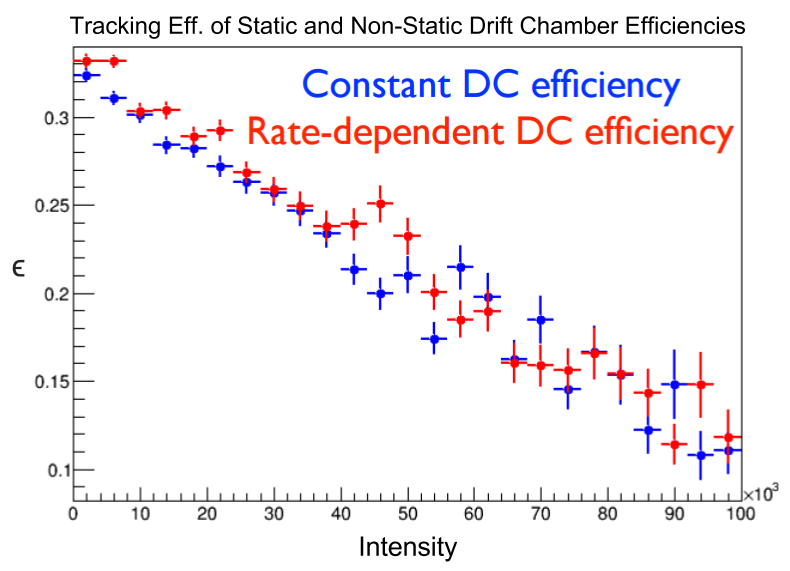
\includegraphics[width=4in]{figures/analysis/ktrack-eff-int.png}
	\caption{The ratio of successful reconstruction to all thrown by MC for two chamber efficiency models. The linear decreases in efficiency are not significantly different from each other.}
	\label{fig:ktrack-eff-int}
\end{figure}

Putting this together:
\begin{itemize}
	\item Differences in chamber efficiency between targets could only come from different resultant chamber occupancies as a result of that target being in the beam's path.
	\item Chamber occupancies are only slightly different for deuterium when compared to the other nuclear targets, and so if efficiencies are different between targets, the modification will likely be very small.
	\item Even in the case of vastly different efficiencies, the tracking efficiency is unchanged.
	\item As a result, effect of chamber efficiency on the yields will be the same for all targets.
	\item $\varepsilon^D/\varepsilon^A$, a measure of how the chamber efficiency effects the deuterium target yields as compared to a nuclear targets, can therefore be considered to be 1.
\end{itemize}

\subsection{Detector Acceptance}

The \emph{true} acceptance as a function of any set of kinematic variables $\bar{x}$ can be expressed as:
\begin{equation}
A(x) = \lim\limits_{N\rightarrow \infty} \frac{Y_{accepted}(\bar{x})}{Y_{thrown} (\bar{x})}\ \ ;\ \ 
N \equiv \int Y_{thrown}(\bar{x}) dx
\end{equation}
where \emph{thrown} denotes Drell-Yan simulated events from Monte Carlo which generates every kinematic value by sampling over the distributions of that variable with a random number generator. The simulation includes such processes as multiple scattering and energy loss that occur due to particle passage through materials (such as our targets and beam dumps). Survey numbers of the experimental hall are used to build an accurate representation of the apparatus and its sensitive detector regions. Muon pairs over much of the kinematic phase space and was weighted according to the known Drell-Yan cross section. This does not factor in any higher order nuclear effects or anything like $\dbar/\ubar$ asymmetries. 

The pairs that qualify as \emph{accepted} are those that satisfy the following two criteria: (1) were able to trace their way through the spectrometer without leaving the sensitive range of the detectors at all stations, and (2) they followed paths that would have satisfied the un-like-sign dimuon trigger (FPGA1). Such data was written to file in a format that matches real experimental data and is then ready for analysis. These events are weighted according to the kinematics and DY cross-section as mentioned above, but for analysis, these weights when analyzed were divided by $N$, the number of thrown events.

Approximately \unit[800,000]{dimuons} were thrown for each target to have the acceptances analyzed. For an absolute acceptance, a study of a full $4\pi$ (or $2\pi$) simulation is required, where $4\pi$ is the solid angle of an entire (semi-)sphere. In such simulations dimuons are thrown in every physically possible direction, and then one can derive the absolute acceptance of the target and/or spectrometer when taking into account this source of \emph{thrown} events. However, for the purposes of these studies, we are only concerned about $\bar{Omega}^D/\bar{Omega}^A$, or the relative acceptance correction. As we see in Fig.~\ref{fig:table-layout}, we see that though the spatial distribution of the liquid deuterium flask and the solid targets are similar, they are fundamentally differently distributed. The density of the deuterium in the flask is constant throughout the length of the flask while the disks are discrete and separated. As a result, it perhaps may be the case that due to beam attenuation, there is a spatial difference between where most dimuons are generated between the different targets. The cause of any acceptance difference, however, is moot; the goal here is to estimate the relative acceptance correction factor between deuterium and the nuclear targets.

The target dependence of the acceptance was studied via yield ratios of heavy targets to that of deuterium for the valid kinematic regions of the experiment. These regions are \unit[4.2]{GeV}$<M_{\gamma^*}<$\unit[10]{GeV}, $0.1<x_2<0.5$, $0.35<x_1<0.9$, $0.0<x_F<0.9$, and \unit[0.0]{GeV}$<p_T<$\unit[3.0]{GeV}. Since no nuclear effects are simulated by the Monte Carlo generator, this ratio should lie at 1; any deviation of this must be purely from the acceptance effects due to the slight differences in the geometries and densities of the targets. The results can be seen in Figure%~\ref{fig:targ-acceptance}.
%\begin{figure}
%	\centering
%	\includegraphics[width=5in]{figures/analysis/targ-acceptance.png}
%	\caption{Ratios of accepted dimuons from heavy targets to deuterium for all kinematic regions of interest.}
%	\label{fig:targ-acceptance}
%\end{figure}
The acceptances of solid targets were calculated by MC to be Z.ZZZ larger than that of the liquid deuterium target. As such, a correction factor of $\bar{\Omega}^A/\bar{\Omega}^D = Z.ZZZ$ is included in the target-to-target normalization.

\section{Dimuon Weights and Corrections}

Weighting of events is a standard procedure for mapping one distribution onto another. The most common example is with Monte Carlo (MC) simulation weighting. A simple physics event MC meant to simulate a well-defined process will `throw' an event with certain kinematics randomly drawn from known distributions via \emph{inverse transform sampling}. By doing this, the simulation is already close to being physical, but according to the cross section of a given process, a certain combination of kinematics will be decidedly more or less probable. A weighting subroutine calculates this likelihood for each event and assigns a weight with respect to how likely that event is based on the kinematics thrown. When binning this weighted data, the adjusted number of events in a bin is given by
\begin{equation}
	N_{bin} = \sum_{i \in bin} w_i\ \ ;\ \ \sigma_{bin} = \sqrt{\sum_{i\in bin} w_i^2}
	\label{eq:gmc-weight}
\end{equation}
which reduces to the Poissonian statistical picture when all weights are 1.

Weighting in this manner can be used in any case where it is desirable to map one distribution to another, as in the case of applying corrections in the case of efficiencies and background subtractions. The most intuitive connection between the use of weights and corrections is in the case of efficiency corrections. Let us say that a dimuon with a certain set of kinematics, for whatever combination of effects, has a reconstruction efficiency of 80\%. This means that four out of five actual dimuons with these kinematics will be reconstructed. If you know this efficiency $\epsilon_{recon}$, you can apply a weight as $w = 1/\epsilon_{recon}$ to each dimuon, as each dimuon represents, in part, a larger population that is not fully represented. In the case of our example, a single dimuon represents $1/0.80 = 1.25$ dimuons in order to make up for the ones that are missed due to that specific inefficiency.

At SeaQuest, there is an issue of rate dependence, and as the sources of this effect is identified, we apply a correction for each source in the form of an applied weight. Here, we discuss the reconstruction efficiency and empty/none target background subtraction corrections.

\subsection{``kEfficiency'' Correction Using Messy/Clean Data}

It is a matter of combinatorics at SeaQuest that, as the intensity increases, the number of background hits on all of the detectors increases. As the number of hits in all the detectors increases, the harder it become for the tracking to identify the actual dimuon(s) from the whole event. This is regarded to be an intensity-dependent tracking efficiency. Seeing as the primary tracking algorithm for SeaQuest is kTracker, this is known as the ``kEfficiency'', and its intensity, target, and kinematic dependency makes it a factor to model and correct for.

The procedure developed by Evan McClellan of UIUC for calculating this kEfficiency is to take compare the performance of the tracking on a clean MC sample of dimuons to an analogous sample that's mixed in with real intensity-dependent background. To do this, a \emph{single} sample of MC-generated dimuons and all of their hits is generated; this sample is denoted as the \emph{``clean''} sample. Then, this sample is mixed with all of the hits from a NIM3 event from the experimental data. The NIM3 trigger, as is discussed in Chapter~2, is the randoms trigger, and by using these events we avoid any effects due to trigger selection bias. This mix of MC dimuons and NIM3 triggered data is denoted as the \emph{``messy''} sample. These NIM3 events all have an intensity, and by embedding a clean MC dimuon into a situation typical of an event at a given intensity, we get a basis by which to judge how efficiently the tracking can reconstruct a dimuon in the clean sample versus the messy sample as a function of intensity (and other kinematic variable).

It is important to note that the DY cross section is so small that there is a negligible chance that a given randomly-triggered NIM3 event will contain an actual dimuon, nonetheless a dimuon matching the characteristics of the MC dimuon that is embedded. As such, it is assumed that the dimuon embedded in the NIM3 event is the only dimuon to find in the event. It is also justified to assume that the kinematics of a dimuon is in no way correlated to the intensity, and the intensity of an event relates only to the amount of background hits observed. The relation to the intensity and the number of background hits can be observed in Figure~\ref{fig:NIM3-Int-Mult}.

\begin{figure}
	\centering
	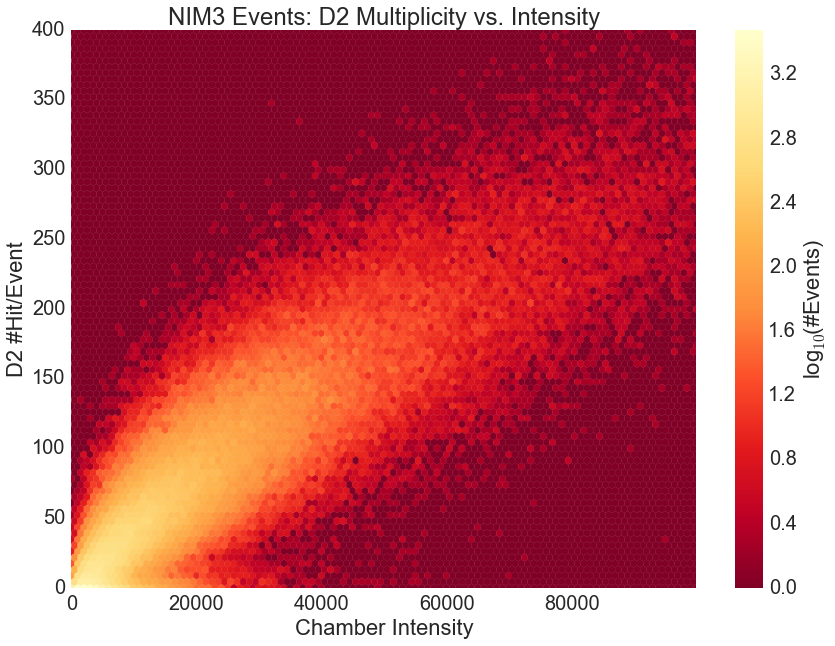
\includegraphics[width=4in]{figures/analysis/NIM3-Int-Mult.png}
	\caption{The linear tendency of detector multiplicity to increase with intensity is observed by looking to unbiased NIM3 events. Here, the occupancy per event of the drift chambers at station 2 are shown as a function of intensity.}
	\label{fig:NIM3-Int-Mult}
\end{figure}

Once the messy and clean samples are prepared, the tracking software is run on them and the two outputs are compared. The first step is to bin the resulting reconstructed dimuons into intensity bins. This binning uses the weights of the dimuons that is assigned by the GMC that created them. The weights are used instead to avoid undue influence on the efficiency from dimuons that are highly unlikely to occur. The value of the bin and its uncertainty are calculated according to Eq.~\ref{eq:gmc-weight}.

For each matching bin, the ratio of $\frac{\#messy}{\#clean}$ values is used to calculate the efficiency of the tracking for that bin. The uncertainty of that efficiency is more complicated, as the relation between the messy and clean samples is of a \emph{binomial} nature. Each dimuon successfully reconstructed in the messy sample represents a \emph{positive} outcome from the number of possible outcomes which is represented by the clean sample. With this kind of relationship, binomial uncertainty calculations must apply. For large enough N number of trials and efficiency $\epsilon\notin \{0,1\}$,
\begin{equation}
\epsilon = \frac{N_+}{N}\ \ ;\ \ \delta\epsilon = \sqrt{\frac{N_+ N_-}{N^3}} = \sqrt{\frac{\epsilon(1-\epsilon)}{N}}
\label{eq:binomial-naive}
\end{equation}
but when weighted trials are involved, things become more complicated in calculating the statistical error. The calculation of this statistical error\cite{blist:binomial} is as follows:
\begin{eqnarray}
	\epsilon & = & \frac{\sum\limits_{i\in+}w_i}{\sum\limits_i w_i} \\
	\delta\epsilon & = & \frac{\sqrt{\sum\limits_{i\in+} w_i^2 \left(\sum\limits_{i\in-} w_i \right)^2 + \
			\sum\limits_{i\in-} w_i^2 \left(\sum\limits_{i\in+} w_i \right)^2}} {\left(\sum\limits_{i}w_i\right)^2}
	\label{eq:binomial-weighted}
\end{eqnarray}
where
\begin{eqnarray}
\sum\limits_{i\in-} w_i & = & \sum\limits_{i\in+}w_i - \sum\limits_{i\in+}w_i \\
\sum\limits_{i\in-} w_i^2 & = & \sum\limits_{i\in+}w_i^2 - \sum\limits_{i\in+}w_i^2 
\end{eqnarray}

For a set of efficiencies, a linear function is fit to the efficiencies. This fit function would then be used to calculate the efficiency for any given dimuon that occurs at any given intensity. The linear parameters are fitted to the data (which is weighted by its statistical uncertainties) by a $\chi^2$-minimization procedure to render a line of best fit along with a confidence interval (Fig.~\ref{fig:keff-all})

\begin{figure}
	\centering
	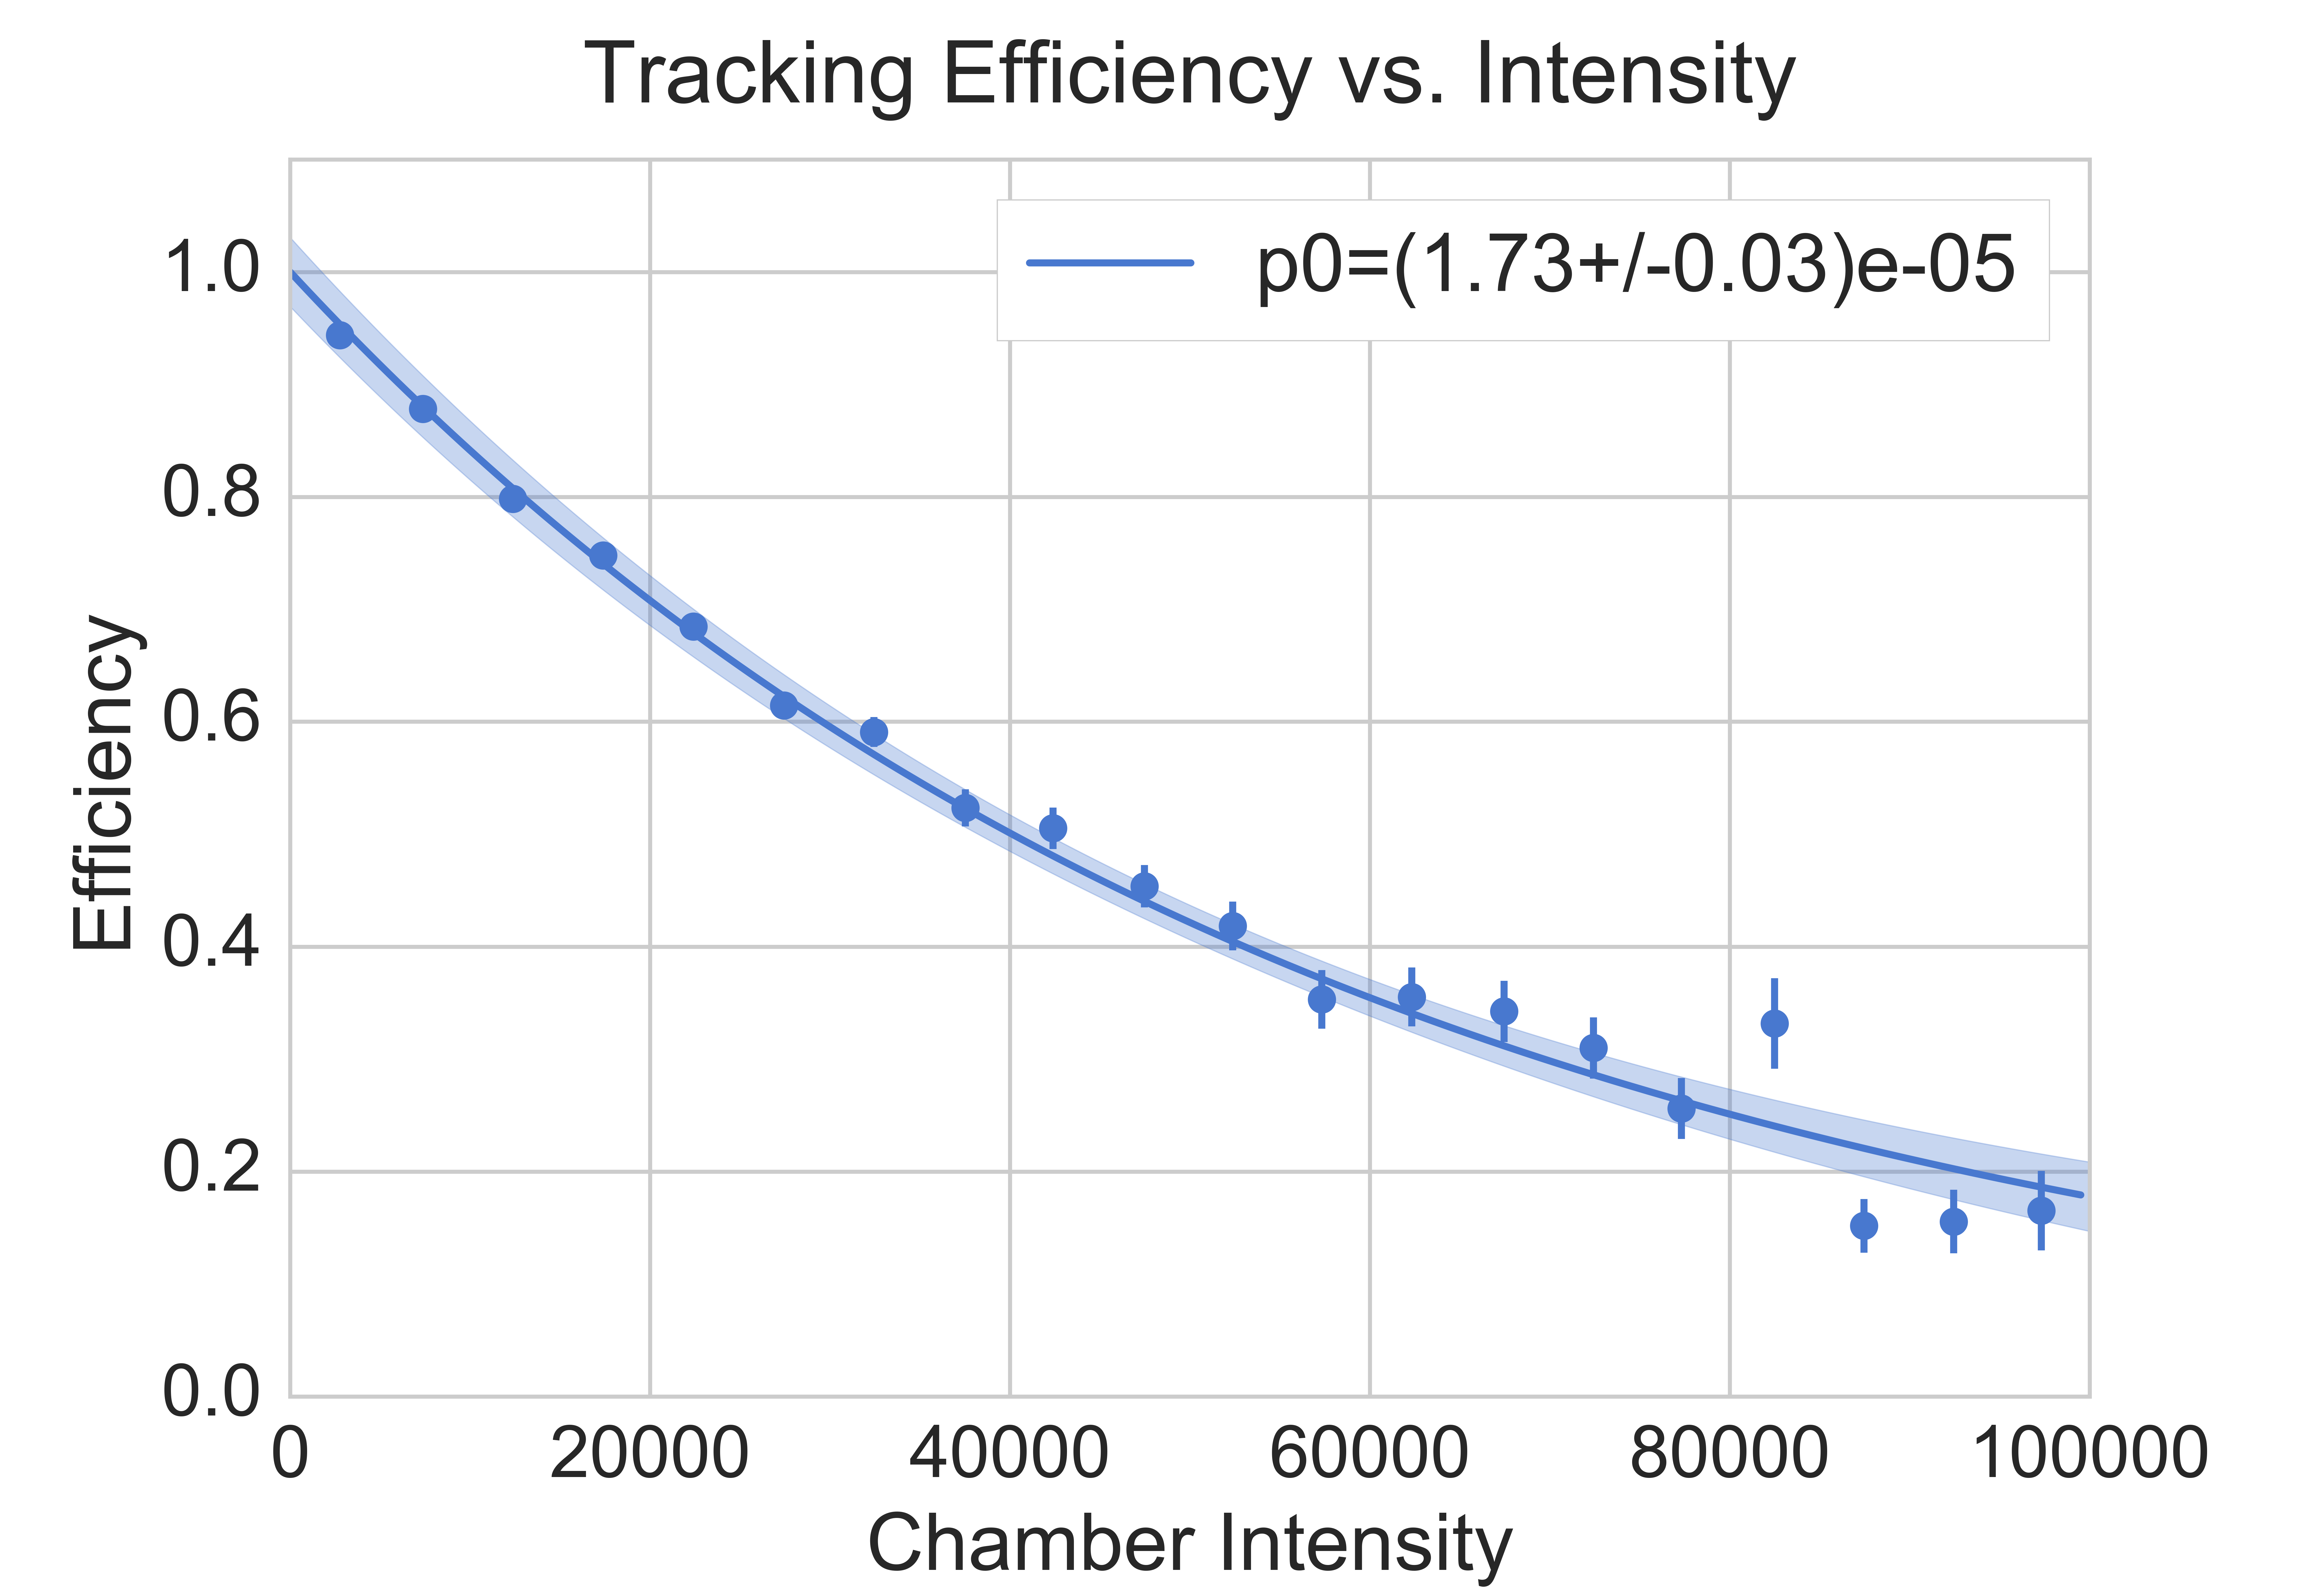
\includegraphics[width=4in]{figures/analysis/all-keff-int.png}
	\caption{The ratio of ``messy'' to ``clean'' dimuon samples from the Deuterium target in Roadset 67 data. This shows the linear relationship of the tracking efficiency to the intensity of the events. The shaded band indicates the 95\% confidence band of the fit.}
	\label{fig:keff-all}
\end{figure}

Further, these fits have a statistically significant kinematic dependence, so it becomes important to unfold the kinematic space and perform this procedure for several kinematic bins in one or more dimensions to assure an accurate efficiency calculation. Of the six defining kinematics of the dimuon, we examine the dependence of the fit on five of them: ($x_1, x_2, p_T, \theta, \phi$), neglecting the azimuthal production angle $\phi_{\gamma^*}$. Each of these five kinematics is divided into three bins (low, medium, high) values to observe on which kinematics the linear fit depends. The results are shown in Figure~\ref{fig:keff-all-kin}.
\begin{figure}
\centering
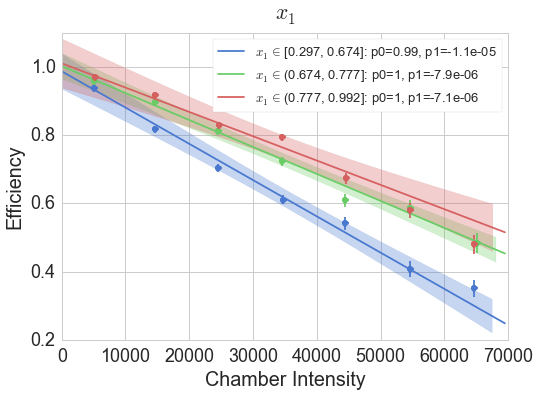
\includegraphics[width=0.49\textwidth]{figures/analysis/x1-keff-int.png}
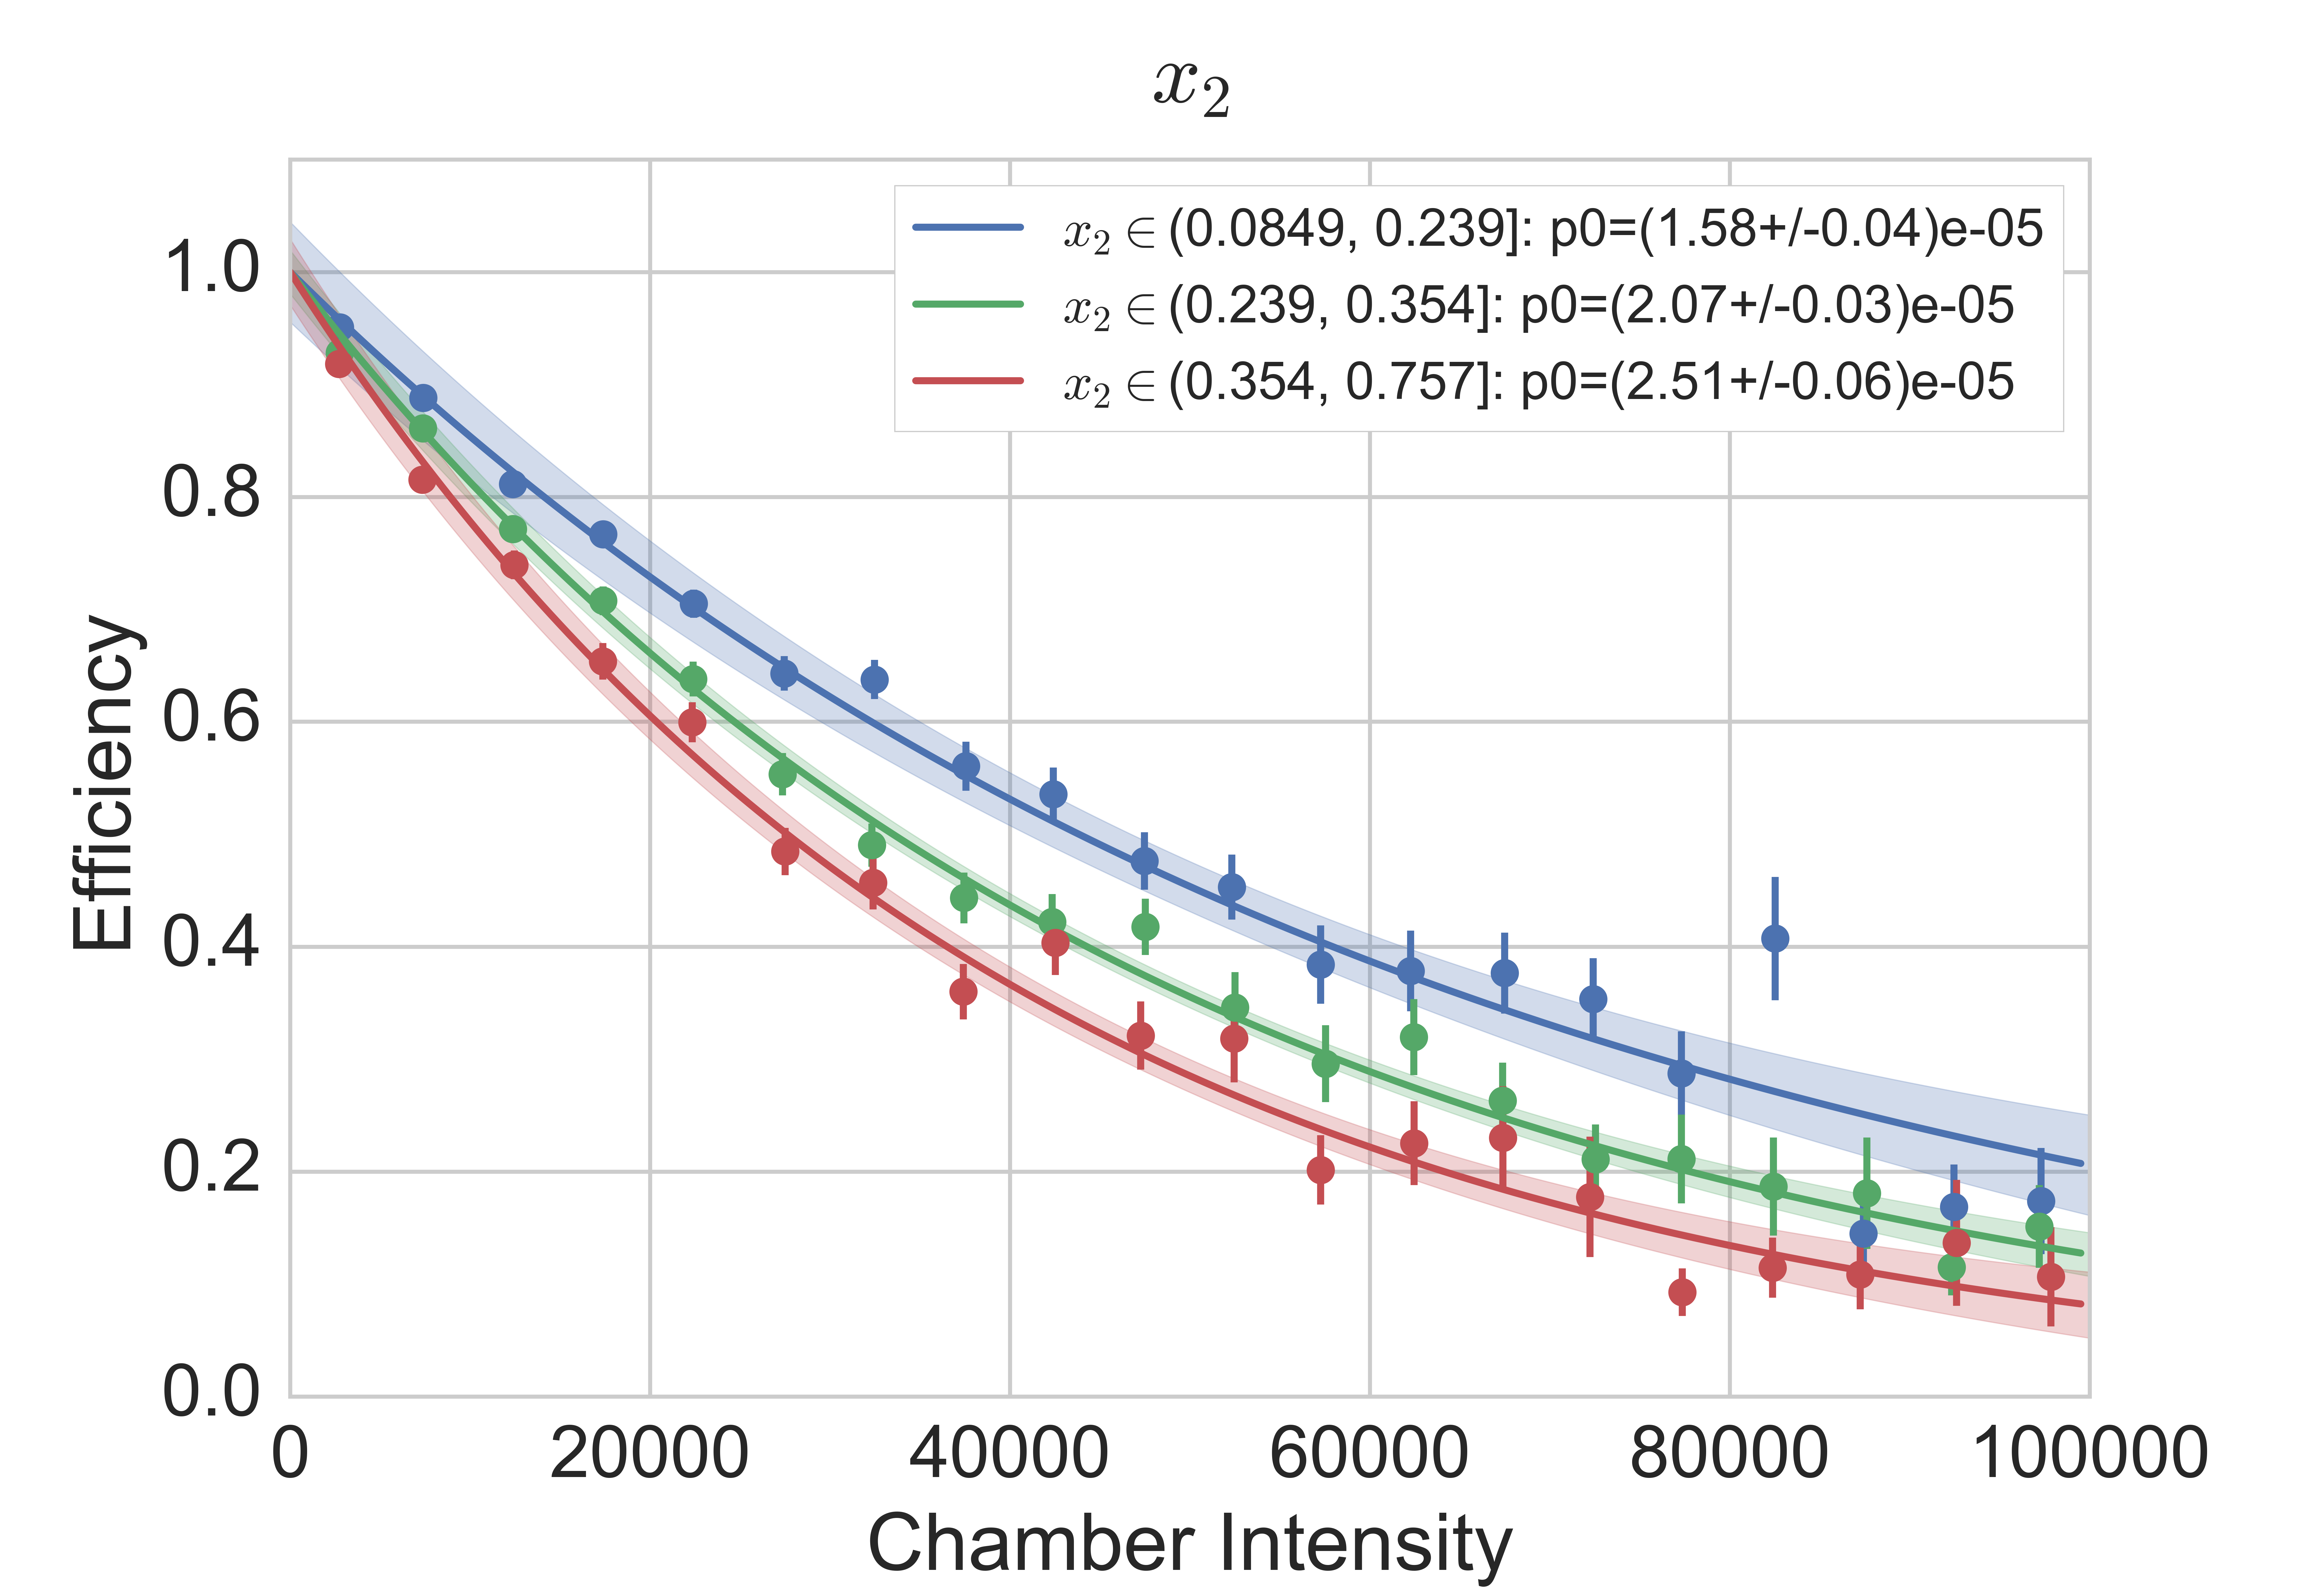
\includegraphics[width=0.49\textwidth]{figures/analysis/x2-keff-int.png} \\ \vspace{20px}
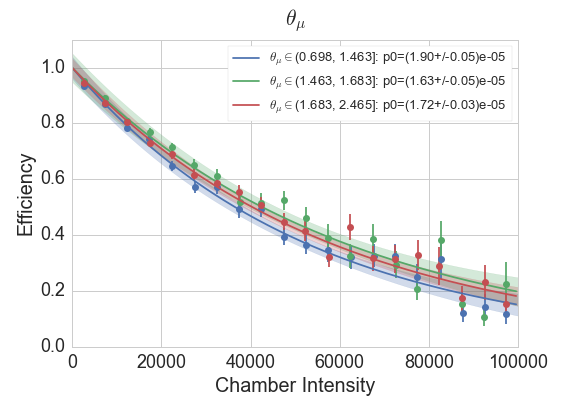
\includegraphics[width=0.49\textwidth]{figures/analysis/theta-keff-int.png}
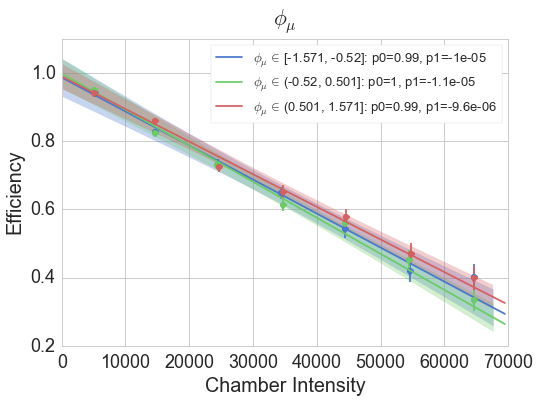
\includegraphics[width=0.49\textwidth]{figures/analysis/phi-keff-int.png} \\ \vspace{20px}
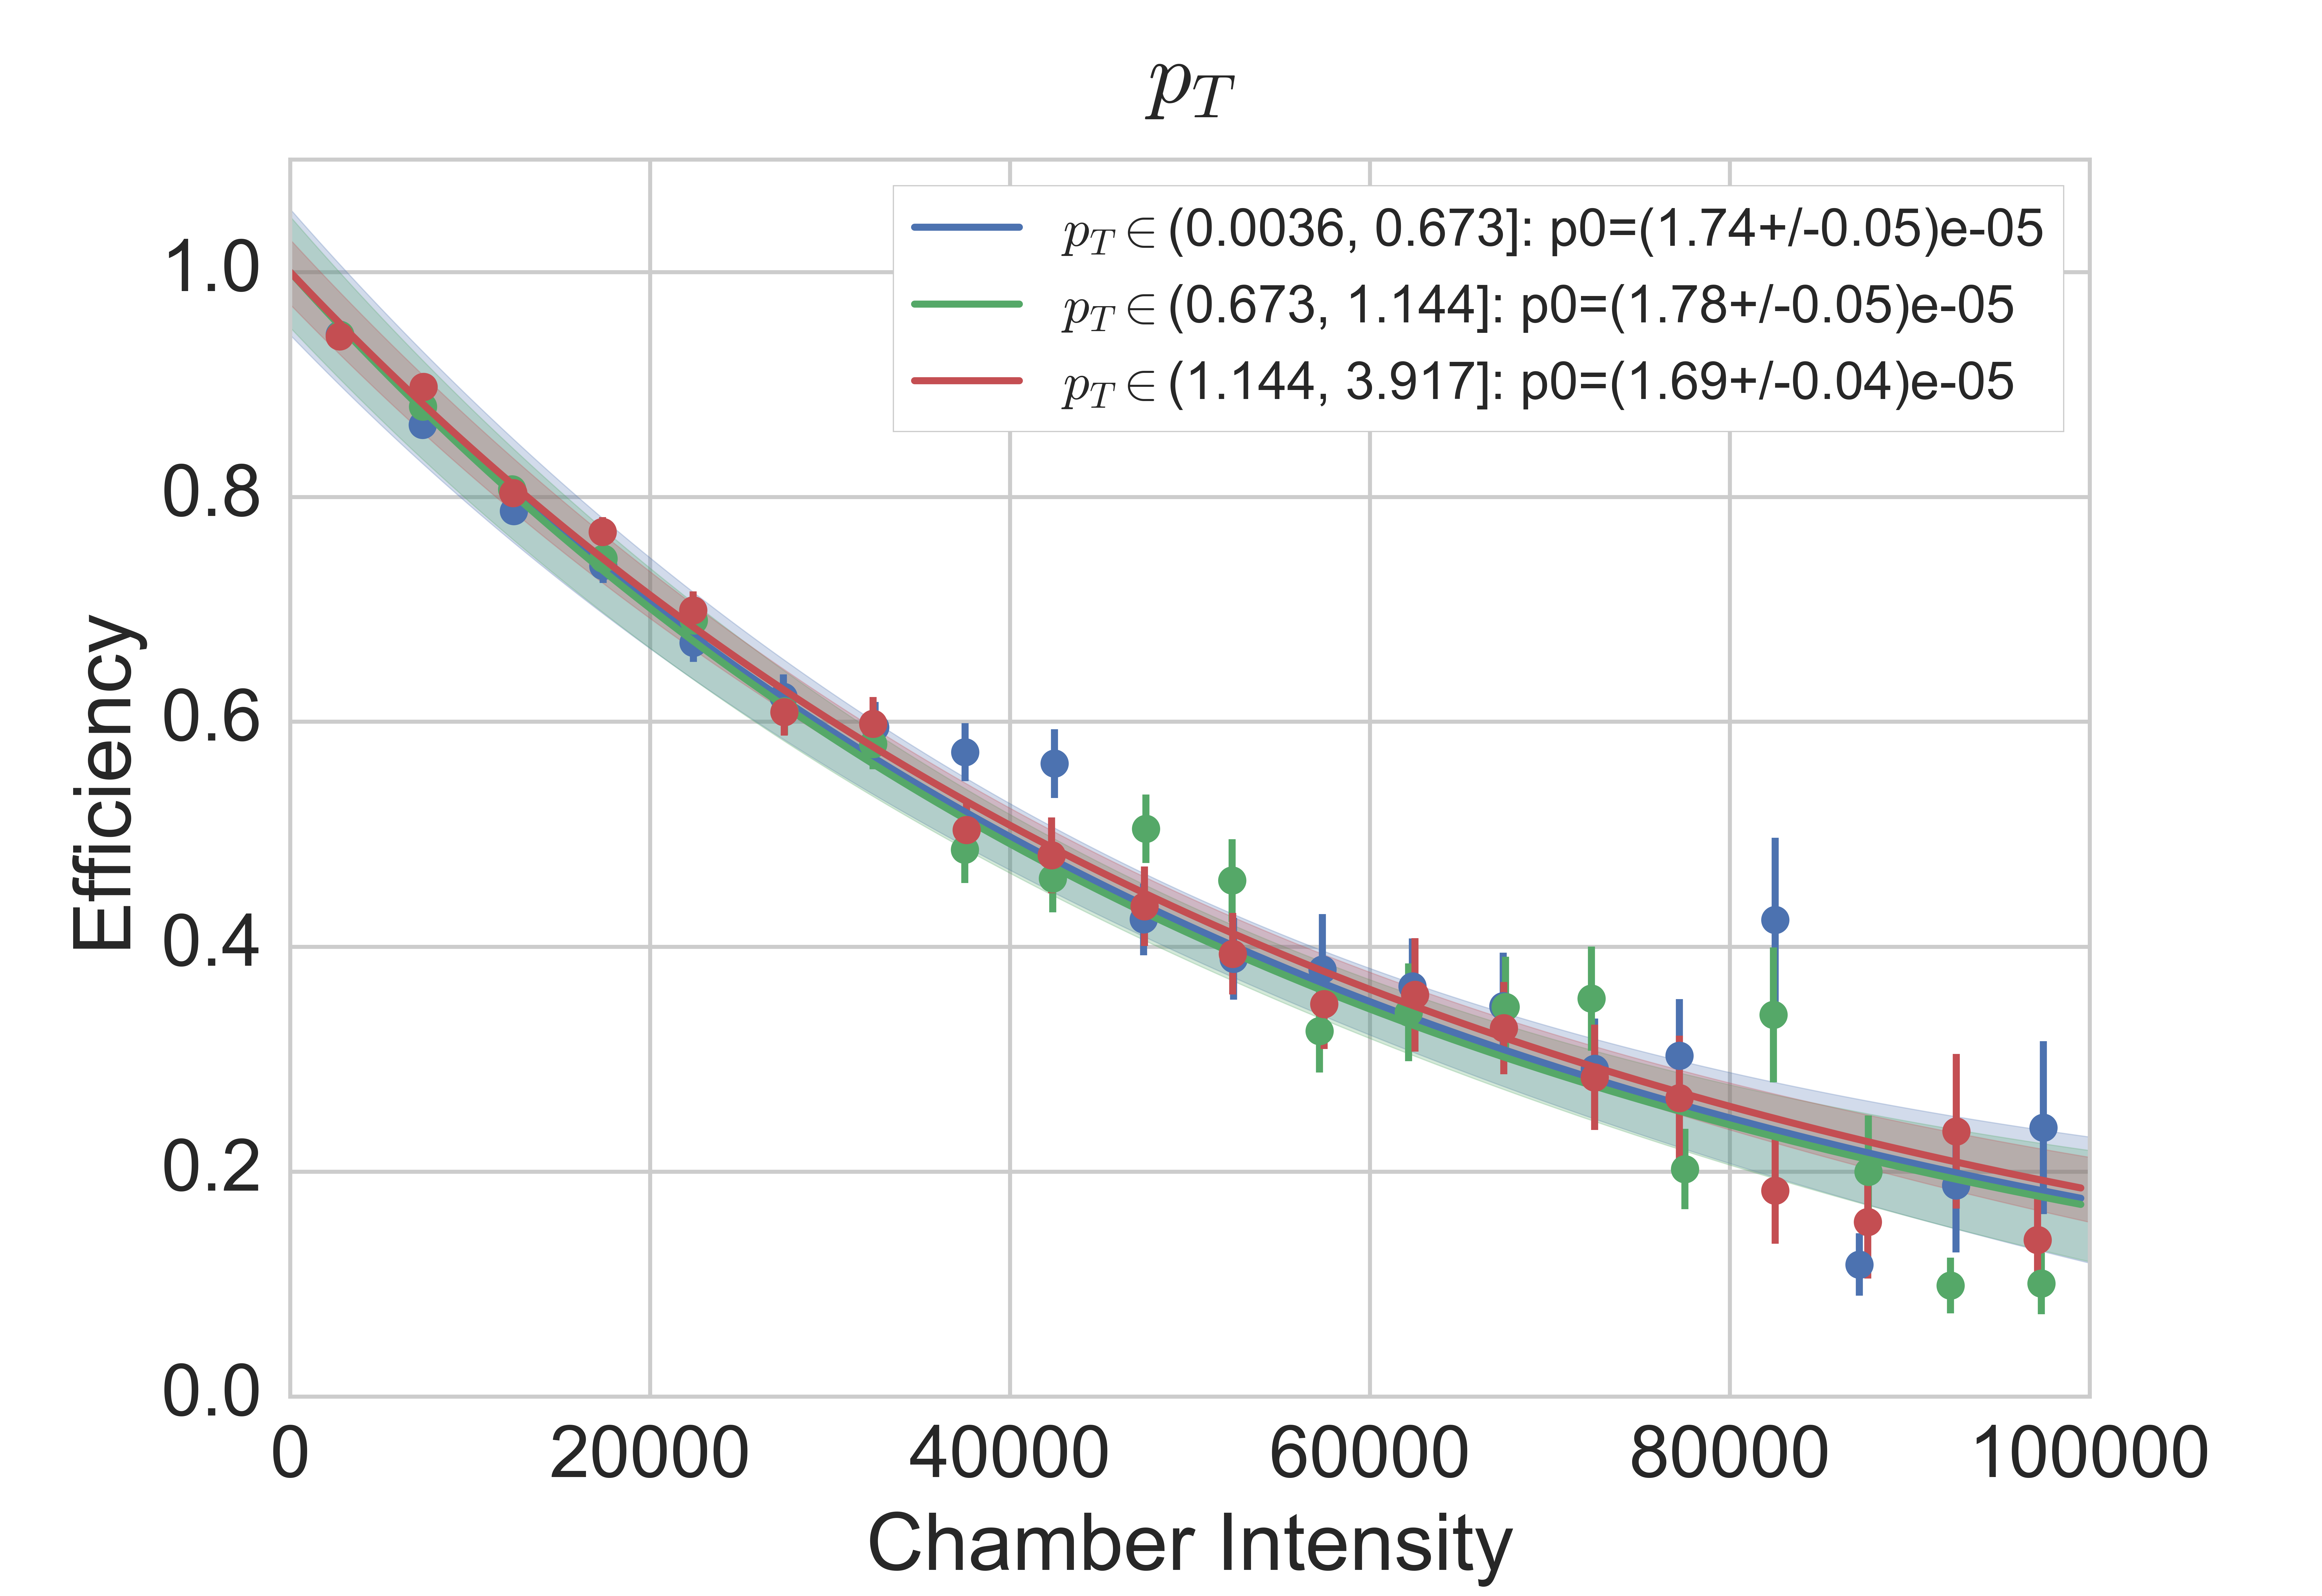
\includegraphics[width=0.49\textwidth]{figures/analysis/pt-keff-int.png} \vspace{10px}
\caption{Tracking efficiency with the data broken into three statistically equivalent bins in the five primary kinematics, ($x_1, x_2, \theta_\mu, \phi_\mu, p_T$). There appears to be a significant kinematic dependence on $x_1$ and $x_2$.}
\label{fig:keff-all-kin}
\end{figure}
The curves produced seem to indicate that there only exists a kinematic dependence on the $x_1$ and $x_2$ kinematics. If this is the case, then the clean and messy samples can be split two-dimensionally in these two kinematics, and a fit can be made to both variables. When analyzing dimuons, its kinematics can indicate which fit to use to calculate the tracking efficiency based on the intensity of the event, and a weight can be calculated.

But before we come to any clear conclusions, let us investigate two more kinematic phase spaces. We know from the discussion in Chapter 1 that \{$x_1, x_2$\} can be used almost interchangeably with \{$x_F, M_{\gamma^*}$\}, and each of $x_1$ and $x_2$ depend on both $x_F$ and $M_{\gamma^*}$. As such, if only one and not the other shows to influence the tracking efficiency curves, then only that one would be needed for the tracking efficiency correction. We see the behavior of the efficiency curves as a function of $x_F$ and $M_{\gamma^*}$ in Figure~\ref{fig:keff-mass-xf}. It can be concluded that since there is no substantial mass dependence observed, the tracking efficiency has a kinematic dependence solely on $x_F$.

\begin{figure}
	\centering
	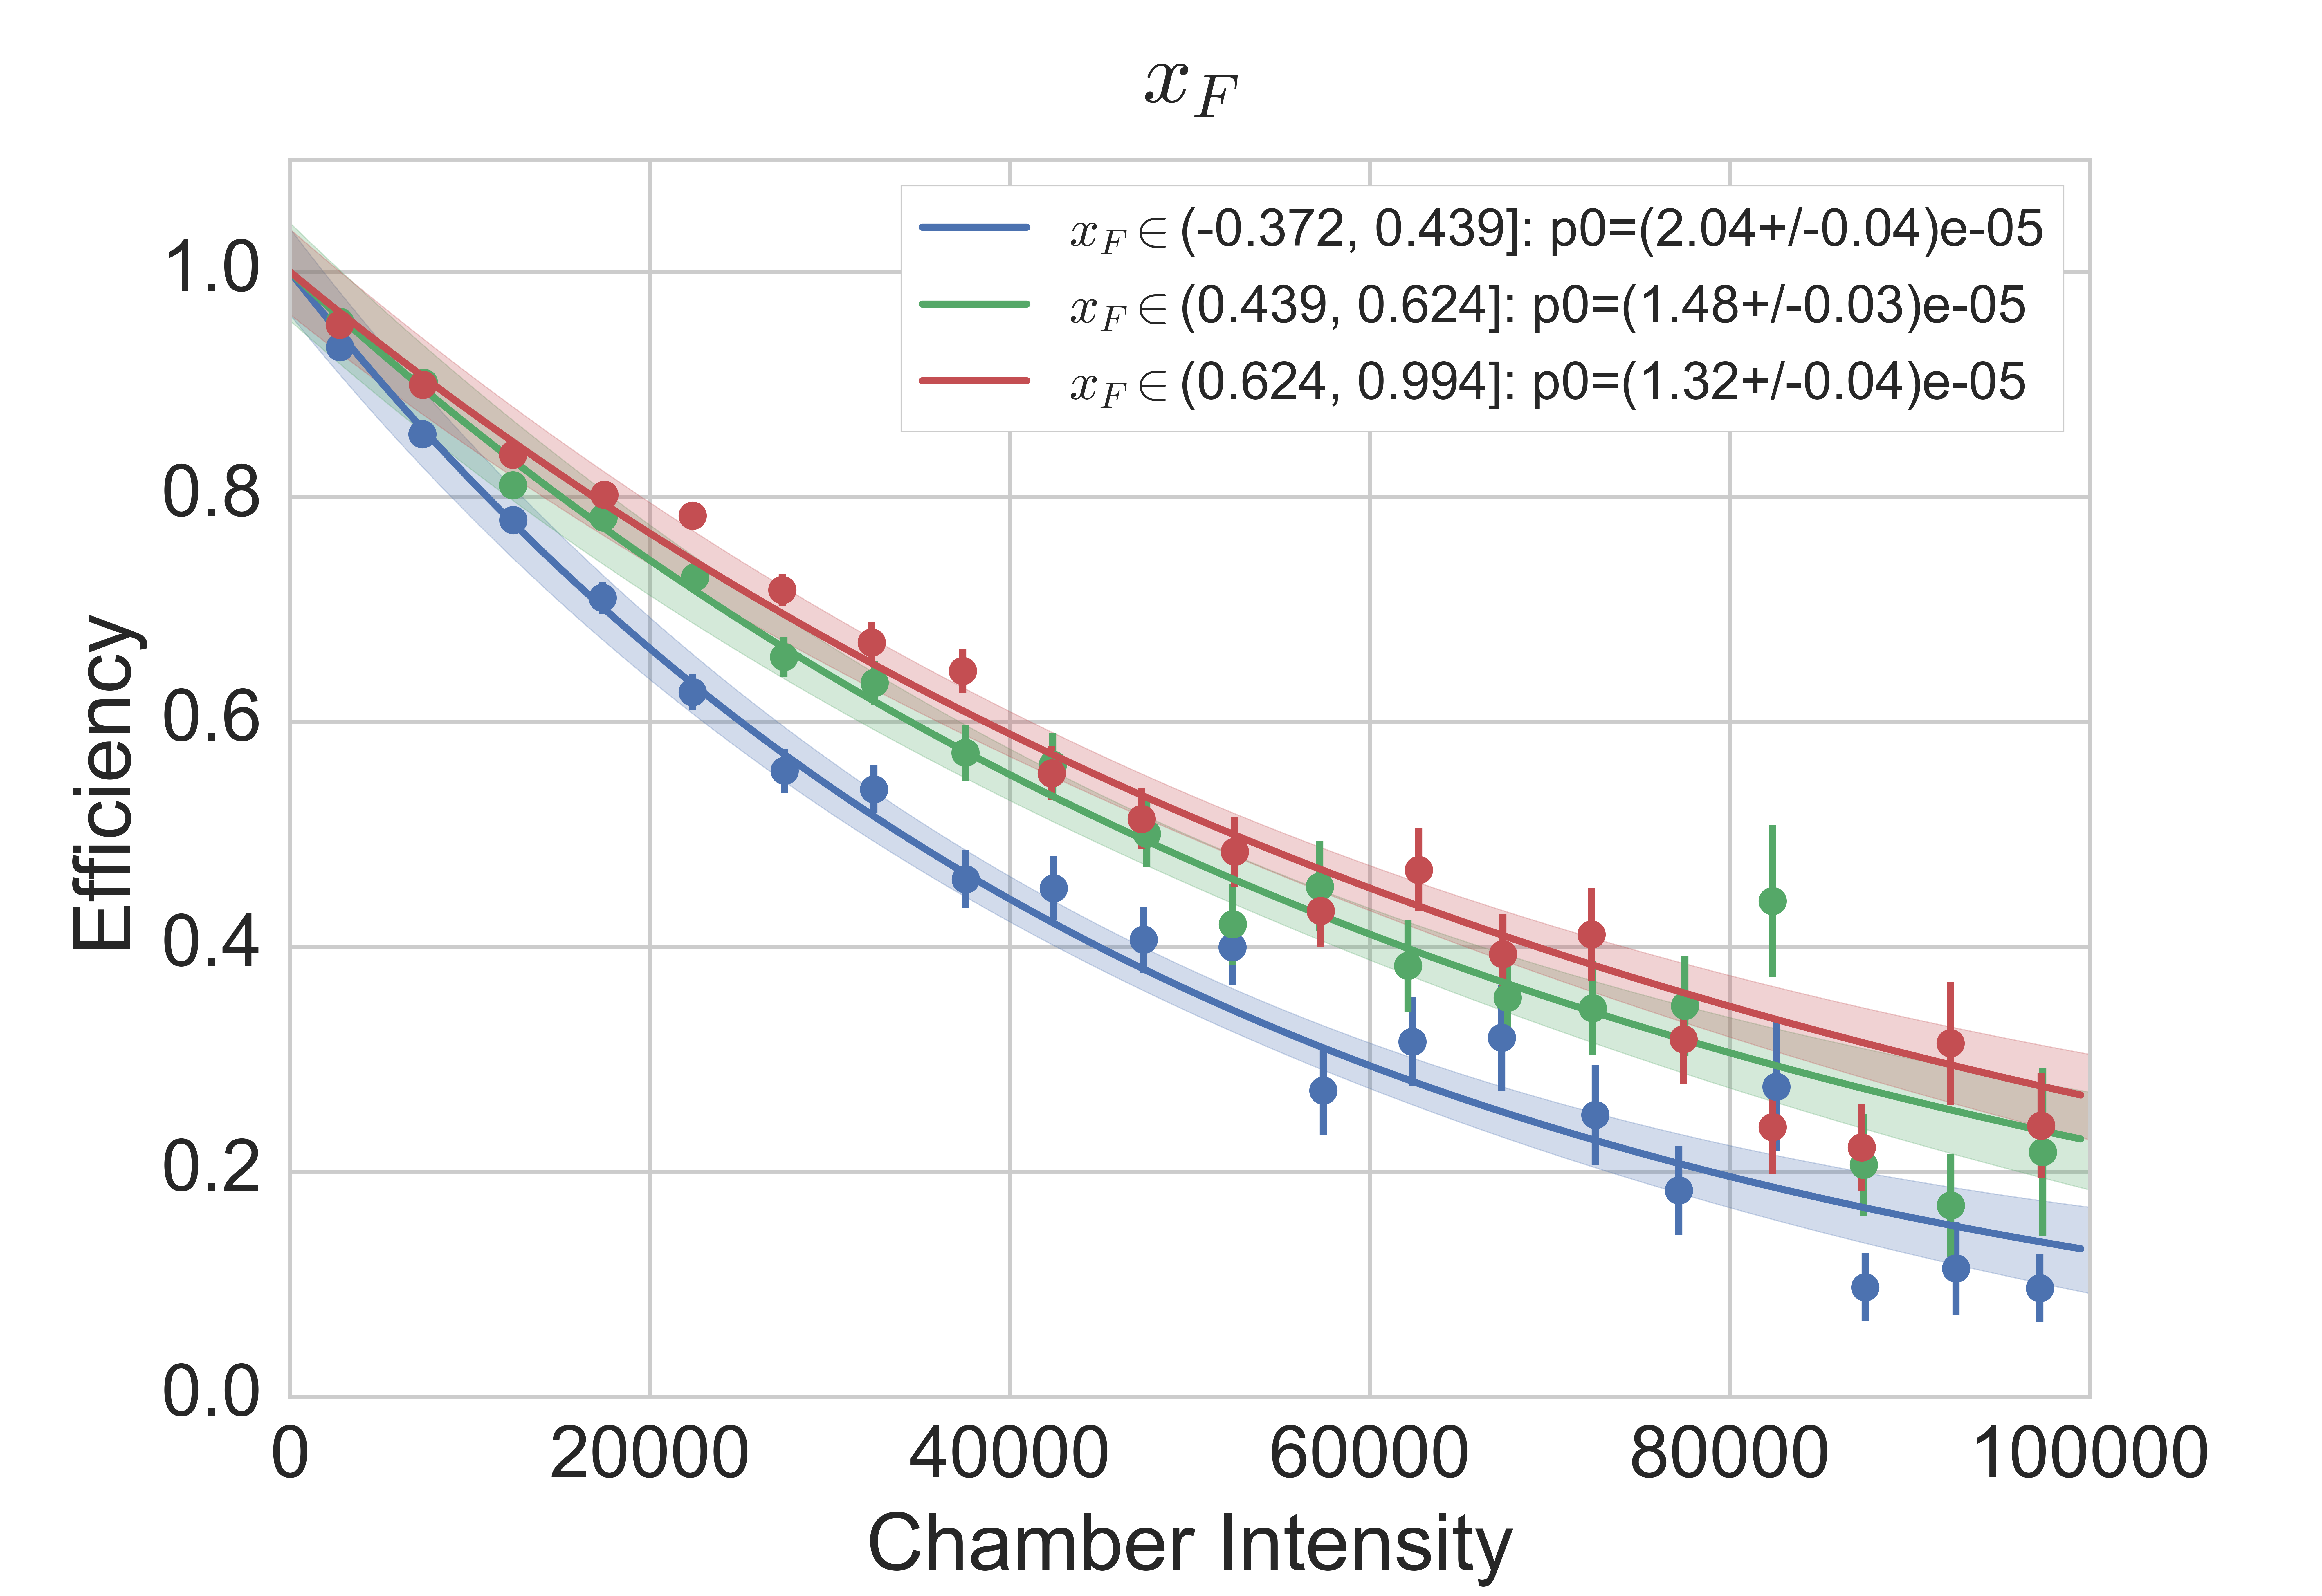
\includegraphics[width=0.49\textwidth]{figures/analysis/xF-keff-int.png}
	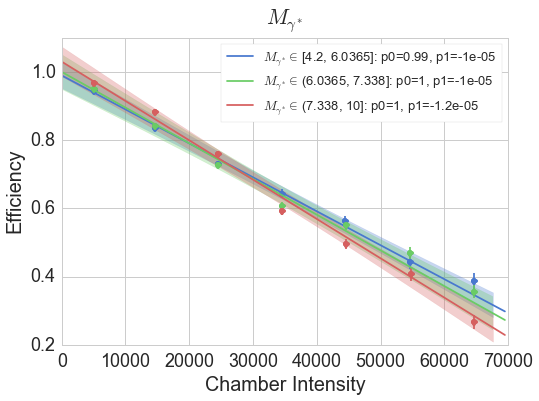
\includegraphics[width=0.49\textwidth]{figures/analysis/mass-keff-int.png}
	\caption{The kinematics $x_F$ and $M_{\gamma^*}$ are investigated. A clear kinematic dependence exists in $x_F$ while $M_{\gamma^*}$ is largely consistent.}
	\label{fig:keff-mass-xf}
\end{figure}

Another consideration is with respect to whether or not there is a target dependence to factor into the correction. For all of the above ``kEfficiency'' plots, only deuterium data is used. The kEfficiency curves for deuterium, hydrogen, carbon, iron, and tungsten can be found on Figure~\ref{fig:keff-target-roadset}. It can be concluded that there is enough of a difference between deuterium, iron, and the rest to justify calculating and applying this correction on a target-by-target basis.
\begin{figure}
	\centering
	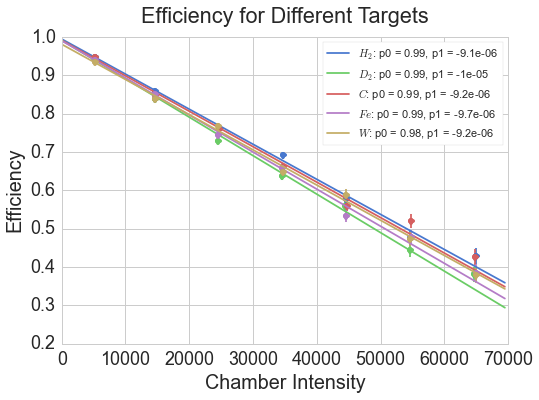
\includegraphics[width=0.49\textwidth]{figures/analysis/target-keff-int.png}
	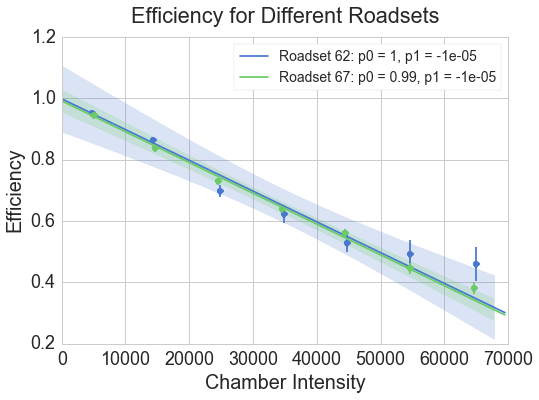
\includegraphics[width=0.49\textwidth]{figures/analysis/roadset-keff-int.png}
	\caption{Comparing the tracking efficiency curves across (left) the five targets and (right) two temporally different subsets (different roadsets) of data. Confidence bands removed from the target plot for the sake of clarity.}
	\label{fig:keff-target-roadset}
\end{figure}

Also, as a sanity check, there should be no time-dependence of this function. A quick check comparing different sets of data from two different roadsets quickly confirm that there is no such time dependence (Fig.~\ref{fig:keff-target-roadset}).

As a result, the final calculation of an tracking efficiency for a given dimuon event should depend on (1) target, (2) $x_F$, and (3) intensity. In order to apply this as a weight, we first define \emph{kEff}$_{t, \bar{x}}(I)$, a set of linear fit functions: one for each target (\emph{t}) and for each kinematic bin ($\bar{x}$), which may be binned in any number of kinematic dimensions. In the case of this analysis, the kinematic binning will only be in $x_F$. The procedure in weighting each dimuon will then be to take each dimuon event \emph{i} and its chamber intensity $I_i$, originating from target $t_i$ in $x_F$ bin $x_{F_i}$, create a weight as
\begin{equation}
w_i = \frac{1}{kEff_{t_i, x_{F_i}}(I_i)}
\end{equation}

\subsection{The Naive Empty Target Correction}

First a few values must be defined. An overall efficiency based on 'contributions' from the Empty/None background can be defined as

\begin{equation}
\epsilon_b = 1 - \frac{Y_b/p_b}{Y_t/p_t} = 1 - \left(\frac{p_t}{p_b}\right) \left( \frac{Y_b}{Y_t} \right)
\end{equation}

where Y is the dimuon \emph{yield} from a given target and \emph{p} is the integrated ``live proton'' count for the same given target. Here, $b \in \{Empty,\ None\}$ and $t\in\{H,\ D,\ C,\ Fe,\ W\}$. It is yet to be conclusively decided by the collaboration whether or not the Empty and None targets are to be combined for these calculations.

The next step is to adjust the yields with the \emph{kEff}$_{t,\bar{x}}(I)$:

\begin{equation}
Y_a \rightarrow Y_a^\prime = \sum_{i:i_t=a} \frac{1}{kEff_{t_i, x_i}(I_i)}
\end{equation}

The yield efficiency when factoring in background then becomes

\begin{equation}
\epsilon^\prime_b = 1 - \left(\frac{p_t}{p_b}\right) \left( \frac{Y^\prime_b}{Y^\prime_t} \right)
\end{equation}

\subsection{Rate Dependent Empty Target Correction}

Upon inspection, the Empty/None target data has shown to exhibit a rate dependence, with many more events per proton being found at higher intensities. This can be corrected for, but the events should first be weighted by their tracking efficiencies. Unfortunately since there are no \emph{messy/clean} embedded data sets for the empty flask, the ``kEfficiency'' fit must be extrapolated from the fits for the deuterium and hydrogen targets. If we are to assume that the difference in fits is a function of the beam's interaction with the target, then we can arrive at the \emph{kEff} exponential fit constants for the empty/none targets ($A_E$) for each kinematic bin from the exponential fit constants from the hydrogen and deuterium targets ($A_{D/H}$). Here, we only additionally need the percentage of beam that interacts with the target ($X_t$), along with a few other values characteristic to the targets found in Table~\ref{tab:targ-details}.
\begin{eqnarray}
X_t & = & 1 - e^{-\frac{L_t}{\lambda_t}} \\
A_E & = & A_H - X_H \cdot \frac{\Delta A}{\Delta X} \\
	   & = & A_H - X_H \cdot \frac{A_D - A_H}{X_D - X_H}
\end{eqnarray}

With this fit constant in hand and the kEfficiency correction applied, one can plot the yields of empty flask and none events as a function of chamber intensity. This plot and its shape can be found in Figure~\red{MAKE FIGURE FOR THIS}. Due to the low-statistics nature of the empty and none events, they are combined across all roadsets and kinematics instead of being broken down. As such, this correction is applied solely based on chamber intensity with no other consideration for roadset or kinematics. The fit that is applied is of the form: $f(I) = p_0 \cdot (1 + p_1 \cdot I_c)$. This form is chosen because the the scale of the final function will be a calculated from the data used, and as such, $p_1$ is the only parameter that is needed. The value calculated was:
\begin{equation}
p_1 = (6.576 \pm 1.566) \times 10^{-5}
\end{equation}
The fit function used, $C_{norm}(I_c) = B \cdot C(I_c) = B \cdot (1 + p_1 \cdot I_c)$  can be interpreted as the probability that a given target dimuon actually arose from something other than a target interaction (beam dump, upstream interactions, flask container). Here, $B$ is the normalization factor, where the condition should stand that the sum of $C_{norm}(I_c)$ over all target dimuons should be equal to the number of events from the empty and none targets. Both sums need to be corrected for kEffeciency and scaled by the number of live protons.
\begin{equation}
\sum\limits_T \frac{B \cdot C(I_c)}{P_T \cdot K_T(I_c)} = \sum\limits_E \frac{1}{P_E \cdot K_E(I_c)}
\end{equation}
\begin{eqnarray}
B & = & \frac{P_T}{P_E} \cdot \frac{\sum\limits_E \frac{1}{K_E(I_c)}}{\sum\limits_T \frac{C(I_c)}{K_T(I_c)}} \\
\delta B & = & \frac{P_T}{P_E} \cdot \frac{\sqrt{\sum\limits_E \frac{1}{K_E(I_c)^2}}}{\sum\limits_T \frac{C(I_c)}{K_T(I_c)}}
\end{eqnarray}

This normalization constant is calculated for each target and each roadset. With this in hand, a weight for correcting for the empty target correction can be applied as $(1 - C_{norm}(I_c))$. One can then combine this with the weighting for the kEffeciency correction (as the weighting should combine multiplicatively):
\begin{equation}
\epsilon_{\text{tot}} = \epsilon_{\text{kEff}} \cdot \epsilon_{\text{empty}} = \frac{1 - C_{norm}(I_c)}{K_T(I_c)}
\end{equation}

It is worth noting that this model does not take into account the attenuation of beam throughout the different target materials, which could alter the scale of the correction slightly. However, without having a figure as to how much of the empty target signal comes from the beam dump and how much of it comes from upstream of the target area, it is currently infeasible to appropriately account for the degree to which a beam attenuation factor should be worked in.

Uncertainties that arise as a result of the uncertainties in the $C(I_x)$ fit and the calculation of $B$ are difficult to propagate analytically. What is performed instead is a an independent variation of $p_1$ and $B$ by $-1\sigma$, 0, and $+1\sigma$ and observing the magnitude of which the per nucleon cross section ratio changes as a result. This systematic uncertainty due to this correction is calculated in the Systematic Uncertainties section of this chapter.

\section{Residual Rate Dependence}

\red{Discuss analysis investigating results for the like-sign reconstruction to estimate the combinatorial background. Hopefully it will be intensity-dependent.}

\section{$LD_2$ Contamination}

\red{Cite Paul's summary of the contamination correction}
During Run III of the SeaQuest experiment, analysis of the deuterium source used indicated that it was impure to a significant degree. This calls for a significant correction since most measurements, yields, ratios, and analyses assume that the targets are pure. An impure deuterium target changes many factors including the averaged mass number of the fluid and its overall density. In this section, the contamination measurements and the correction procedure is discussed.

\subsection{Contamination Measurements}

The SeaQuest deuterium target was emptied and filled several times during data taking. At each of these times, a sample was taken from either the target or from the deuterium gas cylinder used to fill the target. These samples were sent to Los Alamos for isotopic analysis where each sample was analyzed twice. The results of these analyses are shown in Table~\ref{tab:deut-contam}. In each case of parallel analyses on a single gas sample, the two results were in agreement. Upon examination of the deuterium compositions, some problems are immediately clear. Specifically, the ratios of $H_2$, $HD$, and $D_2$ are different between the three samples, but the bottles were supposed to have been filled from the same source many years ago. Second, the some of samples had a significant contribution of other gases, including $N_2$ and $O_2$. This indicates an additional contamination of air. A sample of the first $H_2$ target was analyzed and found to be $\sim98\%$ pure with negligible contributions from other species.

\begin{table}
	\centering
	\begin{tabular}{@{}rrrrrrrrrr@{}}
		\toprule
		{} & \textbf{Runs:} & \multicolumn{2}{c}{3230-11143} & \phantom{abc} & \multicolumn{2}{c}{11144-11477} & \phantom{abc} & \multicolumn{2}{c}{11478-14652} \\ \cmidrule{3-4} \cmidrule{6-7} \cmidrule{9-10}
		\textbf{Species:} & \textbf{Test:} & \multicolumn{1}{c}{1} & \multicolumn{1}{c}{2} & & \multicolumn{1}{c}{1} & \multicolumn{1}{c}{2} & & \multicolumn{1}{c}{1} & \multicolumn{1}{c}{2} \\ \midrule
		$H_2$	& & 1.23 & 1.225 					& & 0.25 & 0.25 				& & 4.603 & 4.591 \\
		$HD$		  & & 16.187 & 16.171 						& & 8.393 & 8.391 			   & & 6.983 & 6.982 \\
		$D_2$ 	& & 79.78 & 79.729 			 	  & & 90.871 & 90.808 			& & 80.504 & 80.443 \\
		$He$ 		   & & 2.20 & 2.188 		 		 	   & & 0.018 & 0.014 				& & $<$0.01 & $<$0.01 \\
		$CH_4$ & & $<$0.009 & $<$0.009 	   & & $<$0.007 & $<$0.007 	 & & $<$0.008 & $<$0.008 \\
		$H_2O$ 	& & $<$0.009 & 0.073   			& & 0.038 & 0.099 			   & & 0.033 & 0.061 \\
		$HDO$ 	 & & 0.015 & 0.026 					& & 0.024 & 0.033 				& & 0.021 & 0.04 \\
		$D_2O$ & & $<$0.007 & $<$0.009      & & $<$0.007 & $<$0.008   & & $<$0.009 & $<$0.012 \\
		$Ne$ 		   & & 0.007 & 0.065 		   		  & & $<$0.027 & $<$0.027 	& & $<$0.03 & $<$0.03 \\
		$N_2$ 	& & 0.428 & 0.419 				    & & 0.323 & 0.323 			   & & 6.395 & 6.382 \\
		$C_2H_6$ & & $<$0.006 & $<$0.006   & & $<$0.005 & $<$0.005   & & $<$0.006 & $<$0.006 \\
		$O_2$ 	& & 0.085 & 0.098 			 	  		   & & 0.068 & 0.068 			   & & 1.389 & 1.416 \\
		$Ar$ 			& & 0.005 & 0.006 				 		  & & 0.004 & 0.003 			  & & 0.063 & 0.064 \\
		$CO_2$ & & $<$0.002 & $<$0.002	    & & 0.011 & 0.009 				 & & 0.01 & 0.01 \\
		$C_3H_8$ & & $<$0.006 & $<$0.006  & & $<$0.005 & $<$0.005   & & $<$0.006 & $<$0.006 \\
		\bottomrule
	\end{tabular}
	\caption{Results of the isotropic analyses of the liquid deuterium samples. Two tests are applied to each sample, and all numbers are in percentages.}
	\label{tab:deut-contam}
\end{table}

The source of the deuterium used at SeaQuest is from a bubble chamber experiment at Fermilab. At some undocumented point in the past, the contents of the bubble chamber were transferred into a tube trailer for storage. At a later time, the $D_2$ was transferred into cylinders for storage. Discussions with gas storage experts indicate that there was likely no special treatment of the cylinders other than being evacuated when they were filled with $D_2$, with the desired special treatment being to ``bake'' the cylinders, or heat them up to release residual hydrogen that tends to diffuse into the metal surface of their inner walls. In addition to that, the containers used to take samples from the target or cylinders were also not ``baked,'' so existing estimates of the contamination may \emph{only} be from the sampling containers -- or the contamination could be doubly worsened by contamination in the sampling containers. As such, effects of this contamination are treated as a systematic error with asymmetric uncertainties. After run 14652, a commercial deuterium gas has been used which has an analyzed purity of $>99.9999\%$, and no systematic uncertainty will need be applied.

Contamination from air in the sample gases is unlikely to have come from the targets. Prior to filling, the targets undergo several cycles of evacuation and refilling with deuterium before the final fill is done. This cycle should flush out all residual air from the target flask. Further, if there was air supply being fed into the target, all but the lowest temperature gases should have been removed by the liquid nitrogen ``cold trap.'' Aside from hydrogen isotopes, helium is the only other component found in the samples. Since the target temperature were approximately \unit[23]{K}, any helium would have been in a gas state and not in the bulk liquid in the flask. Thus, the gases from the analysis shown in Table~\ref{tab:deut-contam} can be renormalized to consider only the hydrogen isotopes, which can be seen in Table~\ref{tab:deut-contam-renorm}.

\begin{table}
	\centering
	\begin{tabular}{@{}rlrrr@{}}
		\toprule
		{} & \textbf{Run} & \multicolumn{1}{c}{3230-} & \multicolumn{1}{c}{11144-} &  \multicolumn{1}{c}{11478} \\ 
		{} & \textbf{Range:} & \multicolumn{1}{c}{11143} & \multicolumn{1}{c}{11477} &  \multicolumn{1}{c}{14652} \\ 
		\textbf{Species:} & & & & \\ \midrule
		$H_2$	& & 1.26   & 0.25  & 4.99 \\
		$HD$    & & 16.65 & 8.44  &	 7.59 \\
		$D_2$ 	& & 82.08 & 91.31 &  87.42 \\
		\bottomrule
	\end{tabular}
	\caption{Renormalized compositions (in percentages) when considering only the hydrogen isotopes.}
	\label{tab:deut-contam-renorm}
\end{table}

Until the true compositions can be ascertained, it has been recommend that analyses use the atomic percentages provided by the Los Alamos analysis as shown in Table~\ref{tab:deut-atomic-perc}, which represents the best understanding of the deuterium at this point. To assign a systematic uncertainty to these numbers, the recommended approach is to use asymmetric uncertainties, assuming that one the extreme values for H and D. Due to the fact that there is a complete inverse correlation between hydrogen and deuterium an uncertainty is assigned to the deuteron percentage only.

\begin{table}
	\centering
	\begin{tabular}{@{}rlrrr@{}}
		\toprule
		{} & \textbf{Run} & \multicolumn{1}{c}{3230-} & \multicolumn{1}{c}{11144-} &  \multicolumn{1}{c}{11478} \\ 
		{} & \textbf{Range:} & \multicolumn{1}{c}{11143} & \multicolumn{1}{c}{11477} &  \multicolumn{1}{c}{14652} \\ 
		\textbf{Atom:} & & & & \\ \midrule
		$H$	& & 9.6   & 4.5  & 8.8 \\
		$D$    & & $90.4^{+5}_{-0}$ & $95.5^{+0}_{-5}$  & $91.2^{+4}_{-1}$ \\
		\bottomrule
	\end{tabular}
	\caption{Atomic percentages of the deuterium targets with asymmetric uncertainties in the $d$ percentage.}
	\label{tab:deut-atomic-perc}
\end{table}

\subsection{Contamination Correction}

With the assumption that the heavier atoms are caught in the cold trap and the gaseous helium stays at the top of the flask and away from the path of the proton beam, a contamination correction is implemented based on the atomic percentage composition detailed in Table~\ref{tab:deut-atomic-perc}. The nuclear interaction length, density, and atomic mass of the liquid deuterium target is corrected based on the cotamination. With $A$ as the atomic mass, $\lambda$ as the nuclear interaction length, $\rho$ as the density, and $F_{H/D}$ as the proportion of $H$ or $D$ in the target, the following are assumed to be approximately true:

\noindent\begin{minipage}{.5\linewidth}
	\begin{eqnarray}
	A & = & A_H\cdot F_H + A_D \cdot F_D \\
	\rho & = & \rho_H\cdot F_H + \rho_D \cdot F_D
	\end{eqnarray}
\end{minipage}%
\begin{minipage}{.5\linewidth}
	\begin{eqnarray}
	\frac{1}{\lambda } & = & \frac{F_H}{\lambda_H} + \frac{F_D}{\lambda_D} \\
	\lambda & = & \frac{\lambda_H \cdot \lambda_D}{F_H \cdot \lambda_D + F_D \cdot \lambda_H}	
	\end{eqnarray}
\end{minipage}
\newline

Due to the contamination, some of the signal events with the liquid deuterium target in place will actually come from hydrogen instead of a deuteron. With $\hat{\sigma}_{pH}$ and $\hat{\sigma}_{pD}$ representing the \emph{measured} target cross section, and $\sigma_{pp}$ and $\sigma_{pn}$ representing the proton-proton and proton-neutron cross section, 

\noindent\begin{minipage}{.5\linewidth}
	\begin{eqnarray}
	\hat{\sigma}_{pH} & = & a \cdot \sigma_{pp} + b \cdot \sigma_{pn} \\
	\hat{\sigma}_{pD} & = & c \cdot \sigma_{pp} + d \cdot \sigma_{pn}
	\end{eqnarray}
\end{minipage}%
\begin{minipage}{.5\linewidth}
	\begin{eqnarray}
	\sigma_{pp} & = & \frac{b \cdot \hat{\sigma}_{pD} - d \cdot \hat{\sigma}_{pH}}{b \cdot c - a \cdot d} \\
	\sigma_{pn} & = & \frac{a \cdot \hat{\sigma}_{pD} - c \cdot \hat{\sigma}_{pH}}{a \cdot d - b \cdot c}
	\end{eqnarray}
\end{minipage}
\newline

\noindent Here, the coefficients $a, b, c,$ and $d$ denote the number of protons and neutrons per atom for the different targets. We know that $a=c=1$, and since the hydrogen target is considered to be pure, $b=0$. The remaining value, $d$, is the fraction of deuteron atoms in the sample ($F_D$ above). With this, we can arrive at an expression for $\sigma_{pD}^{\text{pure}}$.
\begin{eqnarray}
\sigma_{pH}^{\text{pure}} & = & p = \hat{\sigma}_{pH} \\
n & = & \frac{\hat{\sigma}_{pD} - \hat{\sigma}_{pH}}{d} \\
\sigma_{pD}^{\text{pure}} & = & p + n \\
\sigma_{pD}^{\text{pure}} & = & \frac{\hat{\sigma}_{pD} - \hat{\sigma}_{pH}\cdot (1-d)}{d}
\end{eqnarray}

In practice, this correction is applied bin by bin, utilizing the weighted dimuon yield for each target in place of $\hat{\sigma}$. The $d$ used depends on the run ranges applicable to the roadset being analyzed, and the values are derived from those in Table~\ref{tab:deut-atomic-perc}.

\section{\texorpdfstring{$x_A$ Nuclear Scaling Variable}{xA Nuclear Scaling Variable}}

When discussing heavy nuclei and, a certain shift in understanding of scaling variables should be considered. The use of the Bjorken-$x$ scaling variable up until now should be noted to be the parton momentum fraction \emph{of the proton} $x_p = Q^2/(2 m_p \omega)$. It has been recently discussed by Frankfurt \& Strikman\cite{Frankfurt:2012qs} and implemented by Hen \emph{et al.}\cite{Hen:2013oha} that the \emph{structure functions of nucleons bound in nuclei should be extracted in the reference frame of the nucleus}. This is done by considering to the $x_A$ scaling variable, defined as:
\begin{equation}
\frac{x_A}{A} = \frac{Q^2}{2q\cdot P_A} \ \ \ ;\ \ \ x_A = \frac{Q^2}{2q\cdot P_A/A} = \frac{AQ^2}{2\omega m_A} = x_p \cdot \frac{A m_p}{m_A}
\end{equation}
where $q$ and $P_A$ are the 4-momentum vectors of the virtual photon and target nucleus respectively, and $m_A$ is the mass of the target nucleus. For the same values of $Q^2$ and $\omega$, $x_A$ differs from $x_p$ by the ratio of the bound nucleon mass to the free mass. Therefore, a cross section measured at $Q^2$ and $\omega$ on a nucleus $A$ will depend on the nucleon structure function evaluated at $x_A$ rather than $x_p$\footnote{This parlance is in terms of DIS and not Drell-Yan, but the final correction factor still stands for Drell-Yan cross-section ratio measurements with $Q^2\rightarrow M_{\gamma^*}^2$ and $\omega \rightarrow$\red{???}}. For converting from the commonly used $x_p$ over to $x_A$ for the different targets, we apply a factor of $\frac{A m_p}{m_A}$, which for deuterium, carbon, iron, and tungsten are \red{AAAAA, BBBBB, CCCCC, and DDDDD, respectively.} 

As a result, this means that the standard EMC cross section ratio is actually proportional to the nucleon structure function in nucleus $A$ evaluated at parton momentum $x_A$ divided by the nucleon structure function in deuterium evaluated at parton momentum fraction $x_D$ ($x_D = 2Q^2/2m_D\omega = x_p \cdot 2m_p/m_D$)\cite{Hen:2013oha}. For a symmetric nuclei, this can be written as:
\begin{equation}
\frac{2}{A} \cdot \frac{\sigma^A_{DY}(x_p, Q^2)}{\sigma^D_{DY}(x_p, Q^2)} = \frac{F_2^A(x_A, Q^2)}{F_2^D(x_D, Q^2)}
\end{equation}
where $\frac{F_2^A(x_A, Q^2)}{F_2^D(x_D, Q^2)}$ is the ratio of structure functions at the same $Q^2$, but at different $x$. Since we want to compare the structure functions at the same parton momentum fractions, we correct this by using
\begin{eqnarray}
\frac{F_2^A(x_A, Q^2)}{F_2^D(x_D, Q^2)} & = & \frac{F_2^A(x_A, Q^2)}{F_2^D(x_A, Q^2)} \cdot \frac{F_2^D(x_A, Q^2)}{F_2^D(x_D, Q^2)} \\
& & \nonumber \\
\frac{F_2^A(x_A, Q^2)}{F_2^D(x_A, Q^2)} & = & \frac{2}{A} \cdot \frac{\sigma^A_{DY}(x_p, Q^2)}{\sigma^D_{DY}(x_p, Q^2)} \cdot \frac{F_2^D(x_D, Q^2)}{F_2^D(x_A, Q^2)}
\label{eq:struc-func-ratio-xA}
\end{eqnarray}
where here we have $\frac{F_2^D(x_D, Q^2)}{F_2^D(x_A, Q^2)}$ as a correction factor to arrive at $\frac{F_2^A(x_A, Q^2)}{F_2^D(x_A, Q^2)}$, which is the ratio of structure functions in the different nuclei evaluated at the same parton momentum fraction (which is what we're looking to extract). The correction factor can be evaluated using well-known parameterizations of the the structure function of the deuteron \red{(see L.W. Whitlow, Phys. Lett. B282 1992 and P.E. Bosted, Phys. Rev. C77 2008)}. In \red{Figure~refAAA}, the correction factor $\frac{F_2^D(x_D, Q^2)}{F_2^D(x_A, Q^2)}$ is shown as a function of $x_p$ for different targets.

In summary, the traditional EMC per-nucleon cross section ratio measurement has yielded a ratio for $\frac{F_2^A(x_A)}{F_2^D(x_D)}$, when what is really desired is $\frac{F_2^A(x_A)}{F_2^D(x_A)}$. The addition of this $\frac{F_2^D(x_D)}{F_2^D(x_A)}$ correction factor is all that is needed to convert the measurement to the desired result. This correction factor will be applied to the SeaQuest result.

\section{\texorpdfstring{Isoscalar Corrections for $^{183}W$ and $^{56}Fe$}{Isoscalar Corrections for W-183 and Fe-56 }}

\red{Give brief correction in approximating n==p conversion. Be sure to show results for both iso-corrected and not!}

For asymmetric nuclei ($N\neq Z$), following Aubert \emph{et al.} and Bodek \emph{et al.}~\cite{Aubert:1983xm, PhysRevLett.50.1431}, an additional isoscalar correction factor ($R_{ISO}$) is applied to the yield ratio, approximating the ratio to a hypothetical nucleus with equal numbers of protons and neutrons ($N=Z=A/2$):
\begin{equation}
R_{ISO}(x) = \frac{A}{2} \cdot \frac{F_2^p(x, Q^2) + F_2^n(x, Q^2)}{Z\cdot F_2^p(x, Q^2) + N\cdot F_2^n(x,Q^2)} = \frac{A}{2} \cdot \frac{1+R_{np}(x, Q^2)}{Z + N\cdot R_{np}(x, Q^2)}
\end{equation}
\begin{equation}
\frac{\sigma^A_{DY}(x_A, Q^2)_{ISO}}{\sigma^D_{DY}(x_A, Q^2)_{ISO}} = \frac{\sigma^A_{DY}(x_A, Q^2)}{\sigma^D_{DY}(x_A, Q^2)} \cdot R_{ISO}(x_A)
\end{equation}
where $F_2^p$ and $F_2^n$ are the free nucleon structure functions and $R_{np}(x,Q^2) = F_2^n(x,Q^2)/F_2^p(x,Q^2)$ ($R_{np}(x)\approx 1 - 0.8 x$). The free nucleon structure functions are extracted from world data on DIS scattering\CN \red{(Bodek Phys Rev D20 1979, Arrington Phys G Nucl Part Phys 36 2009)} off of deuterium and hydrogen with corrections accounting for Fermi motion of nucleons in deuterium.

Applying this correction to the structure function ratio extracted in Equation~\ref{eq:struc-func-ratio-xA}, the same extraction for asymmetric nuclei becomes \red{(add vertical space between equations.)}
\begin{eqnarray}
\frac{F_2^A(x_A, Q^2)}{F_2^D(x_A, Q^2)} & = & \frac{2}{A} \cdot \frac{\sigma^A_{DY}(x_p, Q^2)}{\sigma^D_{DY}(x_p, Q^2)} \cdot \frac{F_2^D(x_D, Q^2)}{F_2^D(x_A, Q^2)} \cdot R_{ISO}(x_A) \\ 
& & \nonumber \\
\frac{F_2^A(x_A, Q^2)}{F_2^D(x_A, Q^2)} & = & \frac{2}{A} \cdot \frac{\sigma^A_{DY}(x_p, Q^2)_{ISO}}{\sigma^D_{DY}(x_p, Q^2)_{ISO}} \cdot \frac{F_2^D(x_D, Q^2)}{F_2^D(x_A, Q^2)} \cdot \frac{R_{ISO}(x_A) }{R_{ISO}(x_p)}
\end{eqnarray}

\section{Summary of Analysis Steps}

Due to the dynamic nature of the SeaQuest analysis at the time of the writing of this document, it is imporant to lay out the precise procedure of the application of all of these analysis steps. This ensures an ability to reproduce results, understand differences between methods, and allows those new to analysis to have a roadmap for getting started with analysis. Pragmatically speaking, the process taken in this analysis going from the raw dimuon yields to the final extraction of $F_2^A(x)/F_2^D(x)$ can be outlined in several finite steps:
\begin{itemize}
	\item Get raw yields after all analysis cuts (Section X).
	\item Get live proton count (Section X).
	\item Calculate the kEfficiency for targets $H_2$, $D_2$, $C$, $Fe$, and $W$ (Section X).
	\item Extrapolate kEfficiency for Empty/None target.
	\item Calculate $C(I_c)$ and $B_T$ empty target correction fit and parameters (Section X).
	\item Calculate weighted yields:
	\begin{equation}
	Y_T^\prime = \sum\limits_T \frac{1 - B_T \cdot C(I_c)}{K_T(I_c)} \ \ ; \ \ \delta Y_T^\prime = \sqrt{\sum\limits_T \left(\frac{1 - B_T \cdot C(I_c)}{K_T(I_c)}\right)^2}
	\end{equation}
	\item \red{???} Adjust yields by combinatoric background correction factor.
	\item Adjust the deuterium yields for the hydrogen contamination (Equation X).
	\item Take ratios of these adjusted yields $Y_A^\prime/Y_D^\prime$
	\item Apply the target-to-target normalization factor to the ratio:
	\begin{equation}
	N_{A/D} =
	\left(\frac{ N_0^D \cdot \text{lt}^D \cdot T^D(\xi)}{N_0^A \cdot \text{lt}^A \cdot T^A(\xi) } \right) \cdot 
	\left( \frac{ 2 \cdot n_D \cdot L^D }{ A \cdot n_A \cdot L^A } \right) \cdot 
	\frac{ \varepsilon^D }{ \varepsilon^A }  \cdot 
	\frac{ \bar{\Omega}^D }{\bar{ \Omega}^A } \cdot 
	\frac{ \epsilon^D }{ \epsilon^A }
	\end{equation}
	\item Apply the $\frac{F_2^D(x_D, Q^2)}{F_2^D(x_A, Q^2)}$ correction factor to the ratio.
	\item With asymmetric nuclei ($^{56}Fe, ^{138}W$), apply $\frac{R_{ISO}(x_A) }{R_{ISO}(x_p)}$ isoscalar correction factor.
\end{itemize}
It is understood that this procedure is general enough that it can be performed with any kinematic binning. Here, the $x_A$ conversion and the isoscalar correction are applied to the calculated, binned, adjusted yield ratios. It is also perhaps suitable to apply these to each event with precise considerations for each event's invariant mass.


\section{Systematic Uncertainties}
